%!TEX TS-program = xelatex
%!TEX encoding = UTF-8 Unicode
%!BIB TS-program = bibtex
%!BIB program = bibtex

% THIS IS SIGPROC-SP.TEX - VERSION 3.1
% WORKS WITH V3.2SP OF ACM_PROC_ARTICLE-SP.CLS
% APRIL 2009
%
% It is an example file showing how to use the 'acm_proc_article-sp.cls' V3.2SP
% LaTeX2e document class file for Conference Proceedings submissions.
% ----------------------------------------------------------------------------------------------------------------
% This .tex file (and associated .cls V3.2SP) *DOES NOT* produce:
%       1) The Permission Statement
%       2) The Conference (location) Info information
%       3) The Copyright Line with ACM data
%       4) Page numbering
% ---------------------------------------------------------------------------------------------------------------
% It is an example which *does* use the .bib file (from which the .bbl file
% is produced).
% REMEMBER HOWEVER: After having produced the .bbl file,
% and prior to final submission,
% you need to 'insert'  your .bbl file into your source .tex file so as to provide
% ONE 'self-contained' source file.
%
% Questions regarding SIGS should be sent to
% Adrienne Griscti ---> griscti@acm.org
%
% Questions/suggestions regarding the guidelines, .tex and .cls files, etc. to
% Gerald Murray ---> murray@hq.acm.org
%
% For tracking purposes - this is V3.1SP - APRIL 2009

\documentclass{sig-alternate-10pt}

\usepackage{todonotes}
\usepackage{float}

\usepackage[utf8]{inputenc}
\usepackage{auto-pst-pdf}
\usepackage{hyperref}
\usepackage{booktabs}
\usepackage[inline]{enumitem}
\usepackage{hyperref}
\usepackage{todonotes}
\usepackage{multirow}

%\usepackage[style=authoryear,natbib=true]{biblatex}
%\usepackage[style=numeric,natbib=true]{biblatex}
%\bibliography{method}

%\setlength{\bibitemsep}{8pt}
%\setlength{\bibhang}{0.2cm}

\begin{document}

\title{Collaborative Home Network Troubleshooting}
%\title{Browsers as a Collaborative Measurement Platform for the Internet's Edge: an Evaluation of Delay Accuracy}
%probing heterogeneous vantage points from the browser
%enabling browsers 
%delay measurements from the browser 
%abusing the webstack for delay measurements 
%leveraging the webstack for delay measurements to arbitrary end points

%\subtitle{[Extended Abstract]
%\titlenote{A full version of this paper is available as
%\textit{Author's Guide to Preparing ACM SIG Proceedings Using
%\LaTeX$2_\epsilon$\ and BibTeX} at
%\texttt{www.acm.org/eaddress.htm}}}
%
% You need the command \numberofauthors to handle the 'placement
% and alignment' of the authors beneath the title.
%
% For aesthetic reasons, we recommend 'three authors at a time'
% i.e. three 'name/affiliation blocks' be placed beneath the title.
%
% NOTE: You are NOT restricted in how many 'rows' of
% "name/affiliations" may appear. We just ask that you restrict
% the number of 'columns' to three.
%
% Because of the available 'opening page real-estate'
% we ask you to refrain from putting more than six authors
% (two rows with three columns) beneath the article title.
% More than six makes the first-page appear very cluttered indeed.
%
% Use the \alignauthor commands to handle the names
% and affiliations for an 'aesthetic maximum' of six authors.
% Add names, affiliations, addresses for
% the seventh etc. author(s) as the argument for the
% \additionalauthors command.
% These 'additional authors' will be output/set for you
% without further effort on your part as the last section in
% the body of your article BEFORE References or any Appendices.

\numberofauthors{5} %  in this sample file, there are a *total*
% of EIGHT authors. SIX appear on the 'first-page' (for formatting
% reasons) and the remaining two appear in the \additionalauthors section.
%
\author{
% You can go ahead and credit any number of authors here,
% e.g. one 'row of three' or two rows (consisting of one row of three
% and a second row of one, two or three).
%
% The command \alignauthor (no curly braces needed) should
% precede each author name, affiliation/snail-mail address and
% e-mail address. Additionally, tag each line of
% affiliation/address with \affaddr, and tag the
% e-mail address with \email.
%
% 1st. author
\alignauthor
Maximilian Bachl\\
    \affaddr{UPMC}
%       \affaddr{4 Place Jussieu}\\
%       \affaddr{75005 Paris, France}\\
%       \email{maximilian.bachl@gmail.com}
\alignauthor
Renata Teixeira\\
    \affaddr{Supervisor Inria Paris}
\alignauthor
Timur Friedman\\
    \affaddr{Supervisor UPMC} 
\and
\alignauthor
Claudio Sacchi\\
    \affaddr{Supervisor UNITN}
\alignauthor
Anna-Kaisa Pietilainen\\
    \affaddr{Advisor Inria Paris}
}

%\alignauthor
%Maximilian Bachl\\
%       \affaddr{Université Pierre et Marie Curie}\\
%       \affaddr{4 Place Jussieu}\\
%       \affaddr{75005 Paris, France}\\
%       \email{maximilian.bachl@gmail.com}
%}
% There's nothing stopping you putting the seventh, eighth, etc.
% author on the opening page (as the 'third row') but we ask,
% for aesthetic reasons that you place these 'additional authors'
% in the \additional authors block, viz.
%\additionalauthors{Additional authors: John Smith (The Th{\o}rv{\"a}ld Group,
%email: {\texttt{jsmith@affiliation.org}}) and Julius P.~Kumquat
%(The Kumquat Consortium, email: {\texttt{jpkumquat@consortium.net}}).}
%\date{30 July 1999}
% Just remember to make sure that the TOTAL number of authors
% is the number that will appear on the first page PLUS the
% number that will appear in the \additionalauthors section.

\maketitle
\begin{abstract}
The web browser has emerged as a promising vantage point for measuring the internet edge. Browsers allows for platform-independent measurements on a large variety of platforms such as laptops, smartphones and tablets and they make the usage of measurement utilities easier as web applications do not require installation. In the past browsers' capabilities for measurements were limited but recent technologies such as WebRTC offer promising new possibilities. 
%Furthermore, browser based measurements are known to add significant overhead. 
In this thesis, first, various web technologies are tested for their feasibility for delay measurements to targets such as the home router, Internet servers and other devices in the home network. Second, the most suitable technologies with the lowest overheads are used to create a prototype of a web based measurement tool which utilizes collaboration between end user devices in the home and lets them perform delay measurements together. After performing a measurement, the utility evaluates the quality of the wireless connection to the home router and gives the user feedback about the user's devices' Internet connectivity. 
\end{abstract}

% A category with the (minimum) three required fields
%\category{H.4}{Information Systems Applications}{Miscellaneous}
%A category including the fourth, optional field follows...
%\category{D.2.8}{Software Engineering}{Metrics}[complexity measures, performance measures]

%\terms{Theory}

%\keywords{ACM proceedings, \LaTeX, text tagging} % NOT required for Proceedings

%\tableofcontents
%\newpage

%\pagenumbering{arabic}

\section{Introduction}

The internet edge has flourished with the spread of mobile devices and of broadband connectivity to homes, and it is getting even more diverse with many Internet-of-Things devices. With such growth and diversity come the complexity of monitoring and management. Getting vantage points to measure the internet edge is a challenge as we must often instrument end devices. First, installing and running measurement software on end devices requires cooperation, and sometimes considerable technical sophistication, from users. Second, the diversity of device operating systems and configurations brings a number of practical issues to develop portable measurement tools.

To address these challenges, a number of tools to measure the internet edge run from within web browsers (for example, Ookla's Speedtest). Running a measurement tool by the  click of an URL is simple enough even for unsophisticated users and the browser abstracts  a lot of the complexity of  porting software to different systems.

The first part of the thesis (\S\ref{sec:delays}) focusses on examining different well-established and new web technologies and their feasibility for performing delay measurements. For this evaluation various measurement methods are tested on different source platforms which means different web browsers and different operating systems. Besides varying the source platform, the evaluation also investigates measurement methods to different targets (e.g.~the home router or a measurement server in the Internet). The results give insight about the most suitable measurement method for each browser, operating system and type of target.  

In the second part (\S\ref{sec:troubleshooting}) the results from this evaluation are used to develop a collaborative home network troubleshooting web page. The vision of this tool is that users visit it in case they encounter Internet connectivity problems or also when everything works as expected because they are curious about their home network setup and their individual devices' performance. When the user has loaded the page he clicks on a button to initiate the measurement. The web page connects to other devices in the household and performs various measurements to the home router, the Internet and peer devices in the home network. After a few seconds, when the measurements are finished, the user sees a graph which visualizes the quality of the connection between the devices in the home network and the Internet. 
% The tool gives the user feedback about his devices' Internet connectivity's quality based on a color code ranging from green for excellent connectivity to red for bad connectivity. 

The main challenge of developing this troubleshooting web page is to find a good set of metrics which reliably indicate network quality based on the results of the delay measurements. For achieving this, two different methods are proposed such as a simple approach which estimates connection quality by ranking the measurement results comparing to other users' results and a statistical approach.

\subsection{Related Work}

Our work is motivated by the need to measure from within the internet edge. A number of previous works have recognized the need for measurement platforms to better cover the internet edge, starting from SatelliteLab~\cite{dischinger_satellitelab:_2008}, which aimed at extending PlanetLab, a global platform for network tests, to include nodes in edge networks. Since then, the networking research and operations communities have deployed a number of systems and platforms to launch measurements from the internet edge. Some groups distribute hardware that users then connect to edge networks---popular examples are RIPE Atlas~\cite{ripe_ncc_ripe_????} and BISmark~\cite{sundaresan_bismark:_2014}; others rely on software that users install directly on their end systems, for example, the Fathom Firefox extension~\cite{dhawan_fathom:_2012} and the Dasu BitTorrent plugin~\cite{sanchez_dasu:_2013}. Many of these systems use M-Lab~\cite{_measurement_????} servers as targets because they are well-provisioned and connected to multiple locations in the Internet. 

Running measurement scripts directly from browsers as we evaluate in this paper eliminates the need to deploy measurement hardware or install measurement software. Hence, a number of tools for users to test their Internet performance take this approach, for instance, Ookla's speedtest~\cite{ookla_speedtest_????}, NDT~\cite{carlson_network_????}, and Netlyzr~\cite{kreibich_netalyzr:_2010-1}.

Despite its promises, running measurement tasks from browsers is far from trivial. Browsers have a limited API, which prevents the execution of many desirable measurements (for example, a simple traceroute is not possible from within a plain web browser). The Fathom Firefox extension~\cite{dhawan_fathom:_2012} addresses this issue by providing an API for in-page Javascript to perform common network measurement tasks, but unfortunately we cannot yet assume that Fathom's measurement API will be widely available. Moreover, previous studies have shown that browsers introduce variable overheads that degrade measurement accuracy~\cite{li_appraising_2013}. In some cases, this overhead may dwarf the value we are trying to infer (\textit{e.g.}, when estimating delays within a home network).

To our knowledge, all existing web based measurement methods can only inform their users about their Internet connection speed as a whole, from the client device to the measurement server. However, they do not communicate to the user if there is actually one specific component, such as the wireless connection to the router, which is the reason for suboptimal Internet speed. 
%The methods we present and evaluate in this paper are an asset to these tools and others that aim at measuring the performance from within edge networks. 

%One issue of making measurements from browsers is the loss in measurement accuracy (as our results in \S\ref{subsec:servers}--\ref{subsec:local} show). Prior work has warned about inaccuracies when running measurements in PlanetLab~\cite{sommers_active_2007} and RIPE Atlas~\cite{holterbach_quantifying_2015}. Most similar to ours is the study by Li et al.~\cite{li_appraising_2013}, which also studies the accuracy of delay measurements from browsers using a large variety of technologies, as for example plug-ins such as Flash or Java and also native technologies like WebSockets. Also Gavaletz et al.~\cite{gavaletz_-browser_2012} use web technologies to perform measurements with the focus is on native browser technologies such as AJAX. We reappraise their results in \S\ref{subsec:servers} in view of today's web technologies. In particular, we remove the analysis of Flash and Java, which are no longer enabled by default, and add the analysis of WebRTC. We also use the more recent high-resolution time API, which is available today. We introduce new methods for performing measurements to cooperative and non-cooperative targets.  In addition to testing Internet delays, we also test the more challenging scenario of local delays (in \S\ref{subsec:local}), where measured values are smaller than the overheads browsers typically introduce.

\section{Appraising browser based methods to measure delay}
\label{sec:delays}
%\subsection{Introduction}

In this section we examine the potential to leverage web browsers as a vantage point to measure from the internet edge. 
As a first step, we focus on evaluating browsers when measuring round-trip times (RTTs), which is the basis for a number of common measurement tasks. 

We assume unmodified browsers without Fathom or any other add-ons to increase the chances of reaching a larger number of users. Edge networks are often behind NATs and it is desirable to enable measurements both to arbitrary servers connected to the Internet and to devices in the local network (either other end devices or the gateway router). 

Li et al.~\cite{li_appraising_2013} as well as Gavaletz et al.~\cite{gavaletz_-browser_2009} evaluated the feasibility of performing delay measurements in browsers comparing a large variety of web technologies, some plug-in based ones like Java and Flash but also native ones such as AJAX and WebSockets. However, since their publication browsers and web technologies have advanced significantly. First, we reappraise their results in view of recent advances in web technology (\S\ref{subsec:servers}). In particular, Flash and Java are no longer enabled in many browsers by default and newer protocols such as WebRTC and WebSockets are starting to see wide adoption. In addition, all modern browsers support high resolution time APIs (using \texttt{window.performance.now}) making accurate (up to microsecond resolution) measurements in the browser possible. We report on a set of controlled experiments (described in \S\ref{subsec:setup}) where we measure the accuracy and overheads of RTT measurements from the most popular browsers (Chrome, Firefox) and operating systems (Linux, OS X, Windows). We compare several methods to measure RTTs (described in \S\ref{subsec:methods}) including Ajax requests, WebSocket, and WebRTC DataChannel. 
%Furthermore we perform each of these measurements in the case of idle browsing and in the case of other webpages being opened in the browser while the measurements are performed. 
%WebSocket is a browser API and protocol providing full-duplex communication channels over a single TCP connection. WebRTC is a newer addition to the browser networking stacks (and still work-in-progress) that provides real-time communication capabilities (audio and video) and a peer-to-peer UDP based data channel for peer-to-peer interactions to the browser.
Second, in our controlled experiments, RTT measurements to arbitrary targets are performed---the typical case of servers in the Internet (\S\ref{subsec:servers}) but also the gateway router and other end devices inside the local network (\S\ref{subsec:local}). We consider two cases for each target: cooperative and non-cooperative. A cooperative target is one where we can install software or about which we have other information (e.g.~knowledge of an accessible URL). We assume no control of non-cooperative targets.%, and hence we cannot assume support for any particular protocol(s) or applications other than some network reachability.  

%Our results reveal that there are significant variations in overhead across different operating systems and similarly, the implementations of various web technologies in the browsers tested are markedly different. This implies that for different OS and browser combinations some measurement methods perform more accurately than others. Furthermore, the results show that measurements to uncooperative targets are feasible and even achieve smaller overhead than cooperative methods when utilized within the home network.


\subsection{Delay Measurement Methods}
\label{subsec:methods}

In this section we describe the three main methods for measuring RTT from the browser that we consider in this paper. The basic idea is to leverage the standard javascript APIs to send small beacons between the measurement client, \emph{i.e.} a browser executing javascript code embedded in a web page, and an arbitrary target in the local network or in the Internet. A single round-trip-time is measured as the delay between the beacon and the response. For precise timings, we rely on \texttt{window.performance.now} javascript API method that provides high-resolution timestamps with microsecond accuracy. Because the first measurement of any method can include the delay of connection setup (e.g. TCP handshake), we always run two measurements at an interval of 200~ms and discard the first result.
%
Suitable javascript APIs  include AJAX (XmlHttpRequest)~\cite{w3c_xmlhttprequest_????}, WebSocket~\cite{w3c_websocket_????} and WebRTC~\cite{w3c_webrtc_????}. We present each API and how they can be used for network delay measurements in the following subsections. 
%At high-level the methods differ in the underlying network protocols they use, and if the target is required to cooperate or not with the measurement client. 
Table~\ref{tab:methods} provides a summary of the methods. % and Table~\ref{tab:support} lists the current browser support.

\begin{table*}[bt]
\
\noindent\makebox[\textwidth]{%
\begin{small}
\begin{tabular}{lllll}
\toprule
\textbf{Method} & \textbf{Specifics} & \textbf{Coop.} & \textbf{Comments} \\
\midrule
AJAX GET/POST/HEAD & :80/?rand=param & yes & cross domain request allowed \\
AJAX GET/POST/HEAD & :80/?rand=param & no & cross domain request forbidden \\
AJAX GET/POST/HEAD & :80/inexistentPath?rand=param & no & provoking 404 \\
AJAX GET/POST/HEAD & :1337/ & no & provoking `connection refused' \\
\midrule
WebSocket & & yes & requires a WebSocket server at the target \\
\midrule
WebRTC & Data Channel & yes & requires a signaling channel to the peer \\
\bottomrule
\end{tabular}
\end{small}}
\caption {Delay measurement methods overview.} 
\label{tab:methods}
\end{table*}


%\begin{table}[thb]
%\label{tab:support}
%\centering
%\begin{small}
%\begin{tabular}{l p{4cm}}
%\toprule
%\textbf{Method} & \textbf{Browser Support} \\
%\midrule
%AJAX & Chrome (1) \newline
%	     Firefox (1.0) \newline 
%	     Internet Explorer (7) \newline
%	     Opera (yes) \newline 
%	     Safari (1.2) \\
%\midrule
%WebSocket & Chrome (16) \newline
%		      Firefox (11.0) \newline
%		      Internet Explorer (10) \newline
%		      Opera (12.10) \newline
%		      Safari (6.0) \\
%\midrule
%WebRTC DataChannel & Chrome (yes) \newline
%					Firefox (yes) \newline
%					Opera (yes) \\
%\bottomrule
%\end{tabular}
%\end{small}
%\caption {Major browser support for the measurement methods.} 
%\label{tab:support}
%\end{table}


\subsubsection{AJAX}

\texttt{XMLHttpRequest} (also known as AJAX request) is a javascript API that provides %client 
functionality for transferring data between a client (a web page) and a server. Despite its name, XMLHttpRequest can be used to retrieve any type of data, not just XML and it fetches the data using HTTP. %, but it also supports other protocols (\textit{i.e.} file and ftp). 
The API is simple: a client creates an \texttt{XMLHttpRequest} object, and calls \texttt{open} to initialize the request---with the target URL and the HTTP method (HEAD, GET, POST)---and \texttt{send} to send the request including optional data in the HTTP request body. HTTP HEAD requests the HTTP headers of the target URL, GET will fetch the complete URL resource, and POST will send data to the URL triggering a HTTP response from the target.

%Under the hoods, the 
Internally, the browser makes a TCP connection to the target (or reuses an existing connection if available),
% as many browsers pool connections to speed up networking), 
sends the HTTP request to the target web server, and parses the HTTP response for the client. The client receives response objects via an asynchronous event handler callback. 
%Due to the TCP connection setup overhead, one should always perform two consecutive RTT measurements and discard the first as it may measure the RTT twice (TCP handshake + HTTP request-response). 
We must be careful not to receive cached replies either from the browser or some proxy on the path. A standard technique to avoid this is to add a random URL parameter to each request URL.

AJAX requests are subject to the browser's same-origin security policy, which restricts how a document or script loaded from one origin can interact with a resource from another origin. In particular, we cannot make AJAX requests to cross-origin targets (\emph{i.e.} to origins other than the one where the javascript making the request comes from). Alternatively, web servers can allow cross-origin requests using Cross-Origin Resource Sharing (CORS) mechanism~\cite{w3c_cors_????}. CORS gives web servers cross-domain access controls, which enable secure cross-domain data transfers.

\textbf{Measuring delay to cooperating target.} In this scenario, we assume that the target is running a web server that is either the script origin (same-origin request) or it has configured cross-origin access with CORS. In this case, we can measure the round-trip-time as explained above.

\textbf{Measuring delay to non-cooperating target.} We consider two cases in this scenario: the target is running a web server or not at the requested port. In the first case, two things can happen: (i) the target does not allow cross-origin access, the AJAX request returns with an error message after the (optional) TCP connection setup and a single HTTP request-response exchange; or (ii) the target allows cross-origin request but the requested resource does not exist, in which case the AJAX request results in 404 error response after the connection setup (optional) and the HTTP request-response. In both cases, we can measure the round-trip-time as the time from the request to the error response, and as above make two requests and use the latter to be sure to factor out the TCP handshake time. Finally, we can also make AJAX requests to targets at arbitrary ports where no web server is running. These requests will fail at the TCP connection setup phase. In this case, we can use the delay to connection error as the RTT measurement (at the transport level in this case, the initial TCP SYN packet from the client triggers a TCP RST from a well-behaving target host). However, when using arbitrary ports in the target URLs, the connection may be dropped by a filtering firewall, so this method may not be able to reach arbitrary targets in the Internet.

\subsubsection{WebSocket}

The WebSocket API enables two-way communication between a client and a cooperating target server.
 %that has opted-in to communications from that code. 
 The WebSocket protocol consists of an opening handshake over HTTP followed by basic message framing, layered directly on top of TCP.

\textbf{Measuring delay to cooperating target.} The cooperating target is expected to run WebSocket server code\footnote{Major HTTP servers such as Apache or NGINX support the WebSocket handshake negotiation and there exists several server side implementations for handling the requests including one for node.js that we use in our experiments.} at the requested URL and is expected to allow requests. The client initiates a \texttt{WebSocket} connection object with the target server URL, and uses the \texttt{send} method to send arbitrary messages to the server. Responses are received via asynchronous event handler callbacks at the client.

\subsubsection{WebRTC}
\label{subsubsec:webrtc}

The latest addition to the browser networking APIs is WebRTC (Web Real-Time Communications), which is a technology that enables Web applications and sites to capture and optionally stream audio and/or video media, as well as to exchange arbitrary data between browsers without requiring an intermediary. The peer-to-peer connections between two browser clients can be made using the \texttt{RTCDataChannel} javascript interface that represents a bi-directional data channel between two peers of a connection. WebRTC DataChannels provide packet-oriented transmission of data over SCTP~\cite{ieee_rfc4960:_????} encapsulated in DTLS~\cite{ieee_rfc4347:_????} over UDP. Hence, a great advantage of this method over the other technologies discussed above is the fact that DataChannels allow for unordered and unreliable transmissions which makes it a good candidate for RTT measurements (\emph{e.g.} avoids inadvertently including TCP retransmissions in the measurements). 

\textbf{Measuring delay to cooperating target.} Both clients that want to establish a WebRTC connection have to be able to communicate over a signalling channel. While the protocol for this signalling channel is not mandated by the specification, usually -- and also in our experiment -- WebSockets are used. After establishing a connection, the signalling channel is not needed anymore and the participants communicate directly over WebRTC using a JavaScript interface that closely resembles the one of WebSockets. 

\subsection{Experimental Setup}
\label{subsec:setup}


In this section we describe our testbed setup to evaluate the usability and accuracy of the various RTT measurement methods. 
%As we have seen in the previous section, 
All the methods incur some protocol overhead,
% (message framing and possibly TCP dynamics), 
and the APIs are based on asynchronous methods and callbacks running on top of a garbage collected javascript engine. Thus the main goal of our controlled experiments is to understand these overheads on various operating system and browsers. In addition, we are interested in measuring not only delays towards arbitrary servers in the Internet, but also local targets.
% inside the local network such as the gateway router or other devices connected to the local network. 
Typical delays inside a local network are in order of milliseconds or less, hence the delay measurements will only be useful if the  overheads are small enough.

\begin{figure}[tbh]
\begin{center}
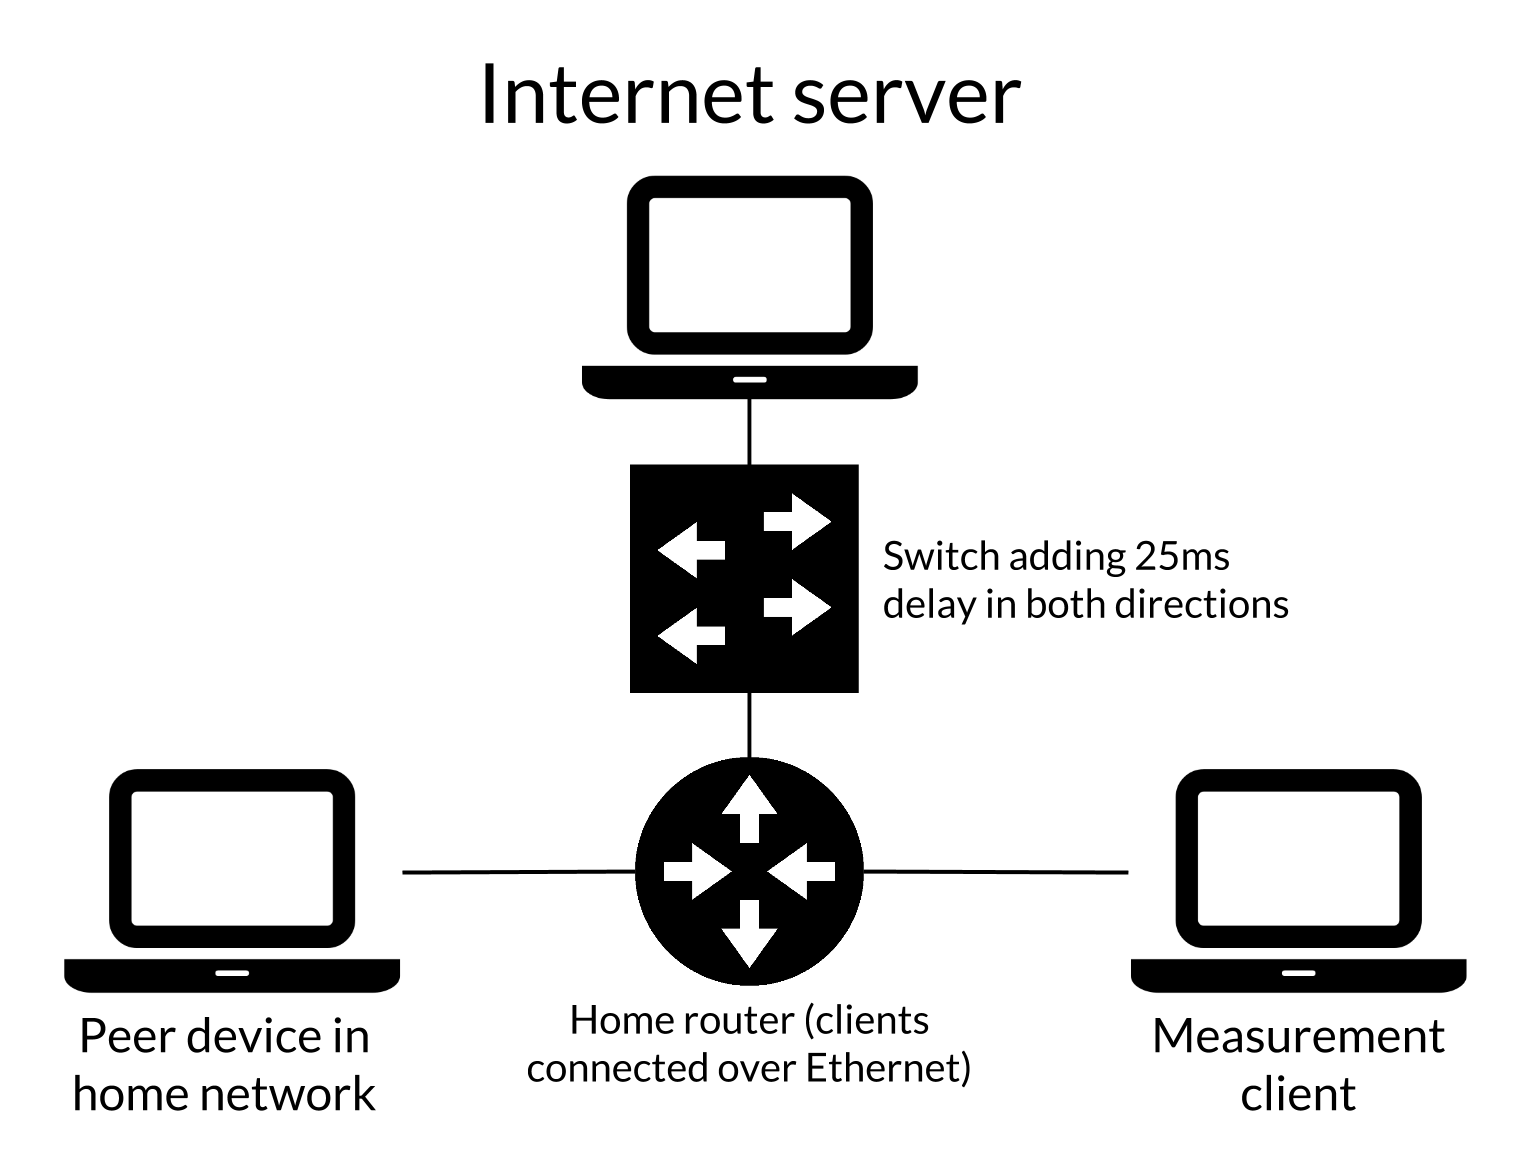
\includegraphics[width=0.65\columnwidth]{figures/setup}
\end{center}
\caption{The testbed setup.}\label{fig:setup}
\end{figure}

Figure~\ref{fig:setup} overviews our testbed. 
The measurement client is a PC running Ubuntu 14.04, OS X El Capitan or Windows 10 with Google Chrome 50 or Mozilla Firefox 45. 
%We test various operating systems and browsers as the implementations of various protocols and the javascript environment are expected to vary from browser to browser. 
Internet Explorer and Safari are excluded due to lack of WebRTC DataChannel support and Opera due to its marginal popularity. 

The measurement client is connected over 100~Mbit/s ethernet to the home router which is a NETGEAR WNDR3700v2 running OpenWRT 15.05. The peer device in the local network is Google Chrome 50 on OS X with 100~Mbit/s ethernet connection to the home router. Finally, the setup has a single controlled Internet server which is a OS X computer connected to the home router over 100~Mbit/s ethernet. To emulate a wide-area link, we place another NETGEAR device acting as a switch between the Internet server and the home router, and use \texttt{netem} to introduce a fixed 25ms delay in both directions (creating an RTT of 50ms between the home router and the Internet server).

\begin{table}[tbh]
\centering
\begin{small}
\begin{tabular}{l l l}
\toprule
\textbf{Target} & \textbf{Technique} & \textbf{Coop.} \\
\midrule
Server & WebRTC DataChannel & yes \\
            & WebSocket & yes  \\
	    & AJAX (GET, POST, HEAD) & yes \\
	    & AJAX (GET, POST, HEAD) & no \\
\midrule
Peer device & WebRTC DataChannel & yes \\
\midrule
Router & AJAX (GET, POST, HEAD) & no \\
\bottomrule
\end{tabular}
\end{small}
\caption {Measurement methods per target.} 
\label{tab:targets}
\end{table}

We have different RTT measurement methods available per target as we summarize in~\autoref{tab:targets}. 
%We test all the available methods to measure the delays to a cooperating Internet server. 
The Internet server runs Apache as a web server and it serves a small one-word document to all the HTTP-based measurement methods. Similarly, we implement a minimal WebSocket server on top of node.js~\cite{node.js_node.js_2016} and use Google Chrome for the WebRTC based experiments. 
%We also test the non-cooperative AJAX methods against the Internet server.
Inside the local network we experiment with WebRTC between the measurement client and the peer device, and the non-cooperative AJAX methods to probe the home router. Note that we could use the non-cooperative AJAX methods to probe any device in the local network, but due to similar rounds-trip-times both to the router and the peer device, we do not repeat the AJAX measurements to the peer device. We did also consider the cooperative router case for AJAX but as we will see in the following sections the non-cooperative AJAX methods offer superior performance. % compared to the cooperative case.

\begin{table}[tbh]
\centering
\begin{small}
\begin{tabular}{llll}
\toprule
OS & Router & Other device & Server \\
\midrule
OS X & {[$0.2$, $0.4$, $0.9$]} & {[$0.3$, $0.6$, $1.0$]} & {[$50.4$, $50.8$, $52.6$]}\\
Ubuntu & {[$0.2$, $0.2$, $0.4$]} & {[$0.3$, $0.6$, $2.1$]} & {[$50.2$, $50.5$, $51.3$]}\\
Win. & {[$0.3$, $0.8$, $1.2$]} & {[$0.5$, $0.9$, $1.4$]} & {[$50.5$, $51.2$, $51.7$]}\\
\bottomrule
\end{tabular}
\end{small}
\caption {Range [min, median, max] of ICMP ping delays (in ms) for each OS in ms.} 
\label{tab:ping_range}
\end{table}

The experiments are executed as follows. Each client (OS + browser, six combinations) executes the measurements in rounds where we perform an RTT measurement using each available method to the three targets (24 method + target combinations in total). We repeat each measurement round 50 times. At the same time of each measurement, we also execute ICMP ping which serve as a baseline. We use the native ping utility on OS X and Linux. However, because Windows' native ping only has millisecond accuracy, we used True Ping~\cite{andrea_denzler_true_2006} on Windows. The baseline RTTs are stable and in expected ranges as we show in Table~\ref{tab:ping_range}.

In the basic experiments we only have a single tab open with a simple empty web page and the embedded javascript code for the measurements. We also test the delay measurements under passive browsing load by opening the 10 most popular web sites in France according to the Alexa ranking~\cite{alexa_top_2016} in background tabs. Our results show that adding load adds 
variation to the distributions of measurement overhead, but does not impact the conclusions, so we omit them from this paper.

\subsection{Internet Delays}
\label{subsec:servers}

In this section we discuss the performance of the browser based delay measurement methods towards Internet targets. This section is partly a reappraisal of the work by Li et al.~\cite{li_appraising_2013} with respect to the cooperative AJAX GET and WebSocket methods. We add the analysis of WebRTC, comparison between additional AJAX methods and AJAX based measurements to non-cooperating targets. In addition, all our results are based on the high-resolution time API that was not available at the time of the previous study.

The basic metric we use throughout the section is the \textit{delay overhead} that we define as the difference between the native ICMP ping measurement and the studied delay measurement method performed at the same time. As discussed before, this overhead accounts for the protocol overhead and any additional delays caused by the browser and its javascript engine. In general, we are after method(s) with low and/or constant delay overhead.

\subsubsection{Cooperating Target}

\begin{figure}[thb]
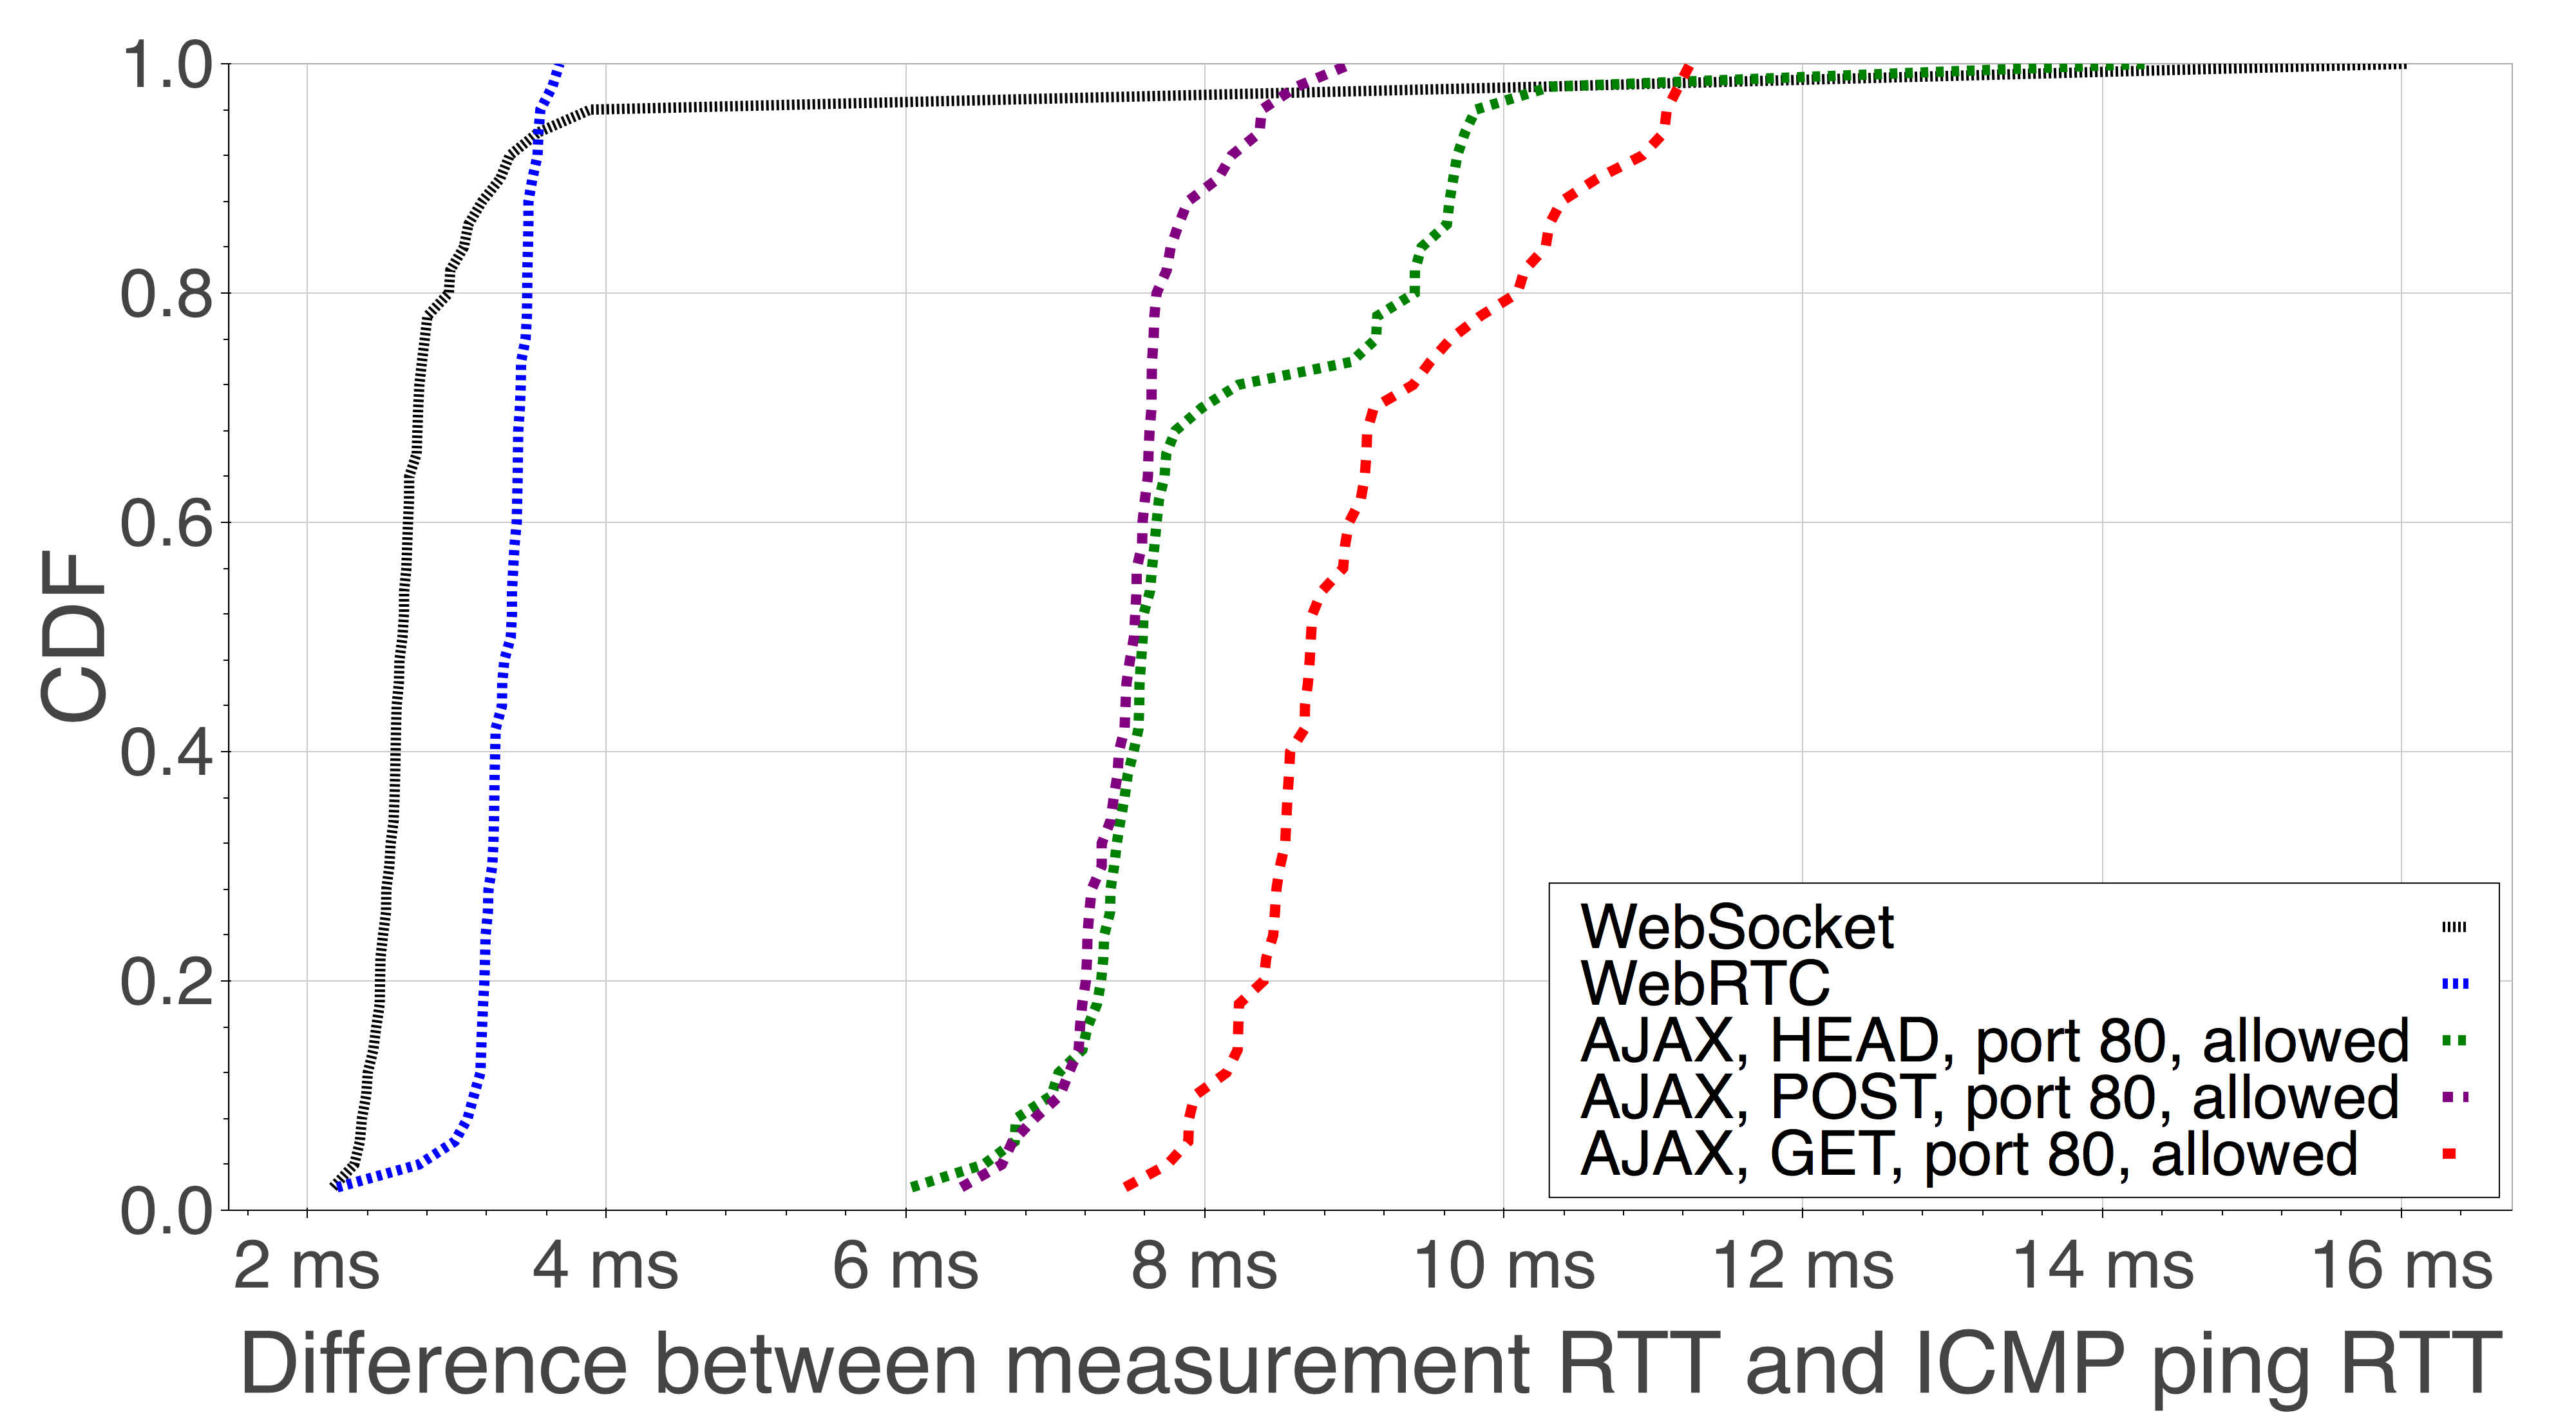
\includegraphics[width=\columnwidth]{figures/inet-coop}
\caption{Delay overheads when measuring a cooperating Internet target (OS X/Chrome).}
\label{fig:inet_coop}
\end{figure}

We plot in Figure~\ref{fig:inet_coop} the delay overhead of the various cooperative measurement methods (the depicted results are from OS X with Chrome, the results are similar for Firefox and other operating systems). The WebSocket method results in the lowest overheads, below 3ms, confirming the findings of Li et al.~\cite{li_appraising_2013}. However, while the WebSocket method generally has a low overhead, we observe a small number of measurements with significantly higher overheads up to 20ms. These occur across all OS and browsers and a further inspection of packet traces reveal that these outliers are not caused by delays in the client browser but rather by a processing delay of up to 20~ms in the WebSocket echo server. These findings are unexpected as our WebSocket server is extremely simple and leverages a widely used library but should be nevertheless taken into account if using WebSockets for delay measurements. Interestingly, the WebRTC method shows rather good and stable performance with only in a slightly higher overhead of above 3ms compared to WebSocket. Moreover, the overhead shows little variance making WebRTC a good candidate for delay measurements with cooperating targets.

The AJAX based methods perform clearly worse due to the HTTP protocol overhead (larger payloads and request + response parsing) and the delay overheads are between 7-9ms in the median case. We compare the HTTP GET, POST and HEAD methods in Figure~\ref{fig:inet_coop}, and observe that POST and HEAD are somewhat better than GET (usually below 8ms overhead compared to more than 8ms), and that POST has additionally lower variance making it the best AJAX based method for delay measurements. 

\subsubsection{Non-cooperating Target}

\begin{figure}[h]
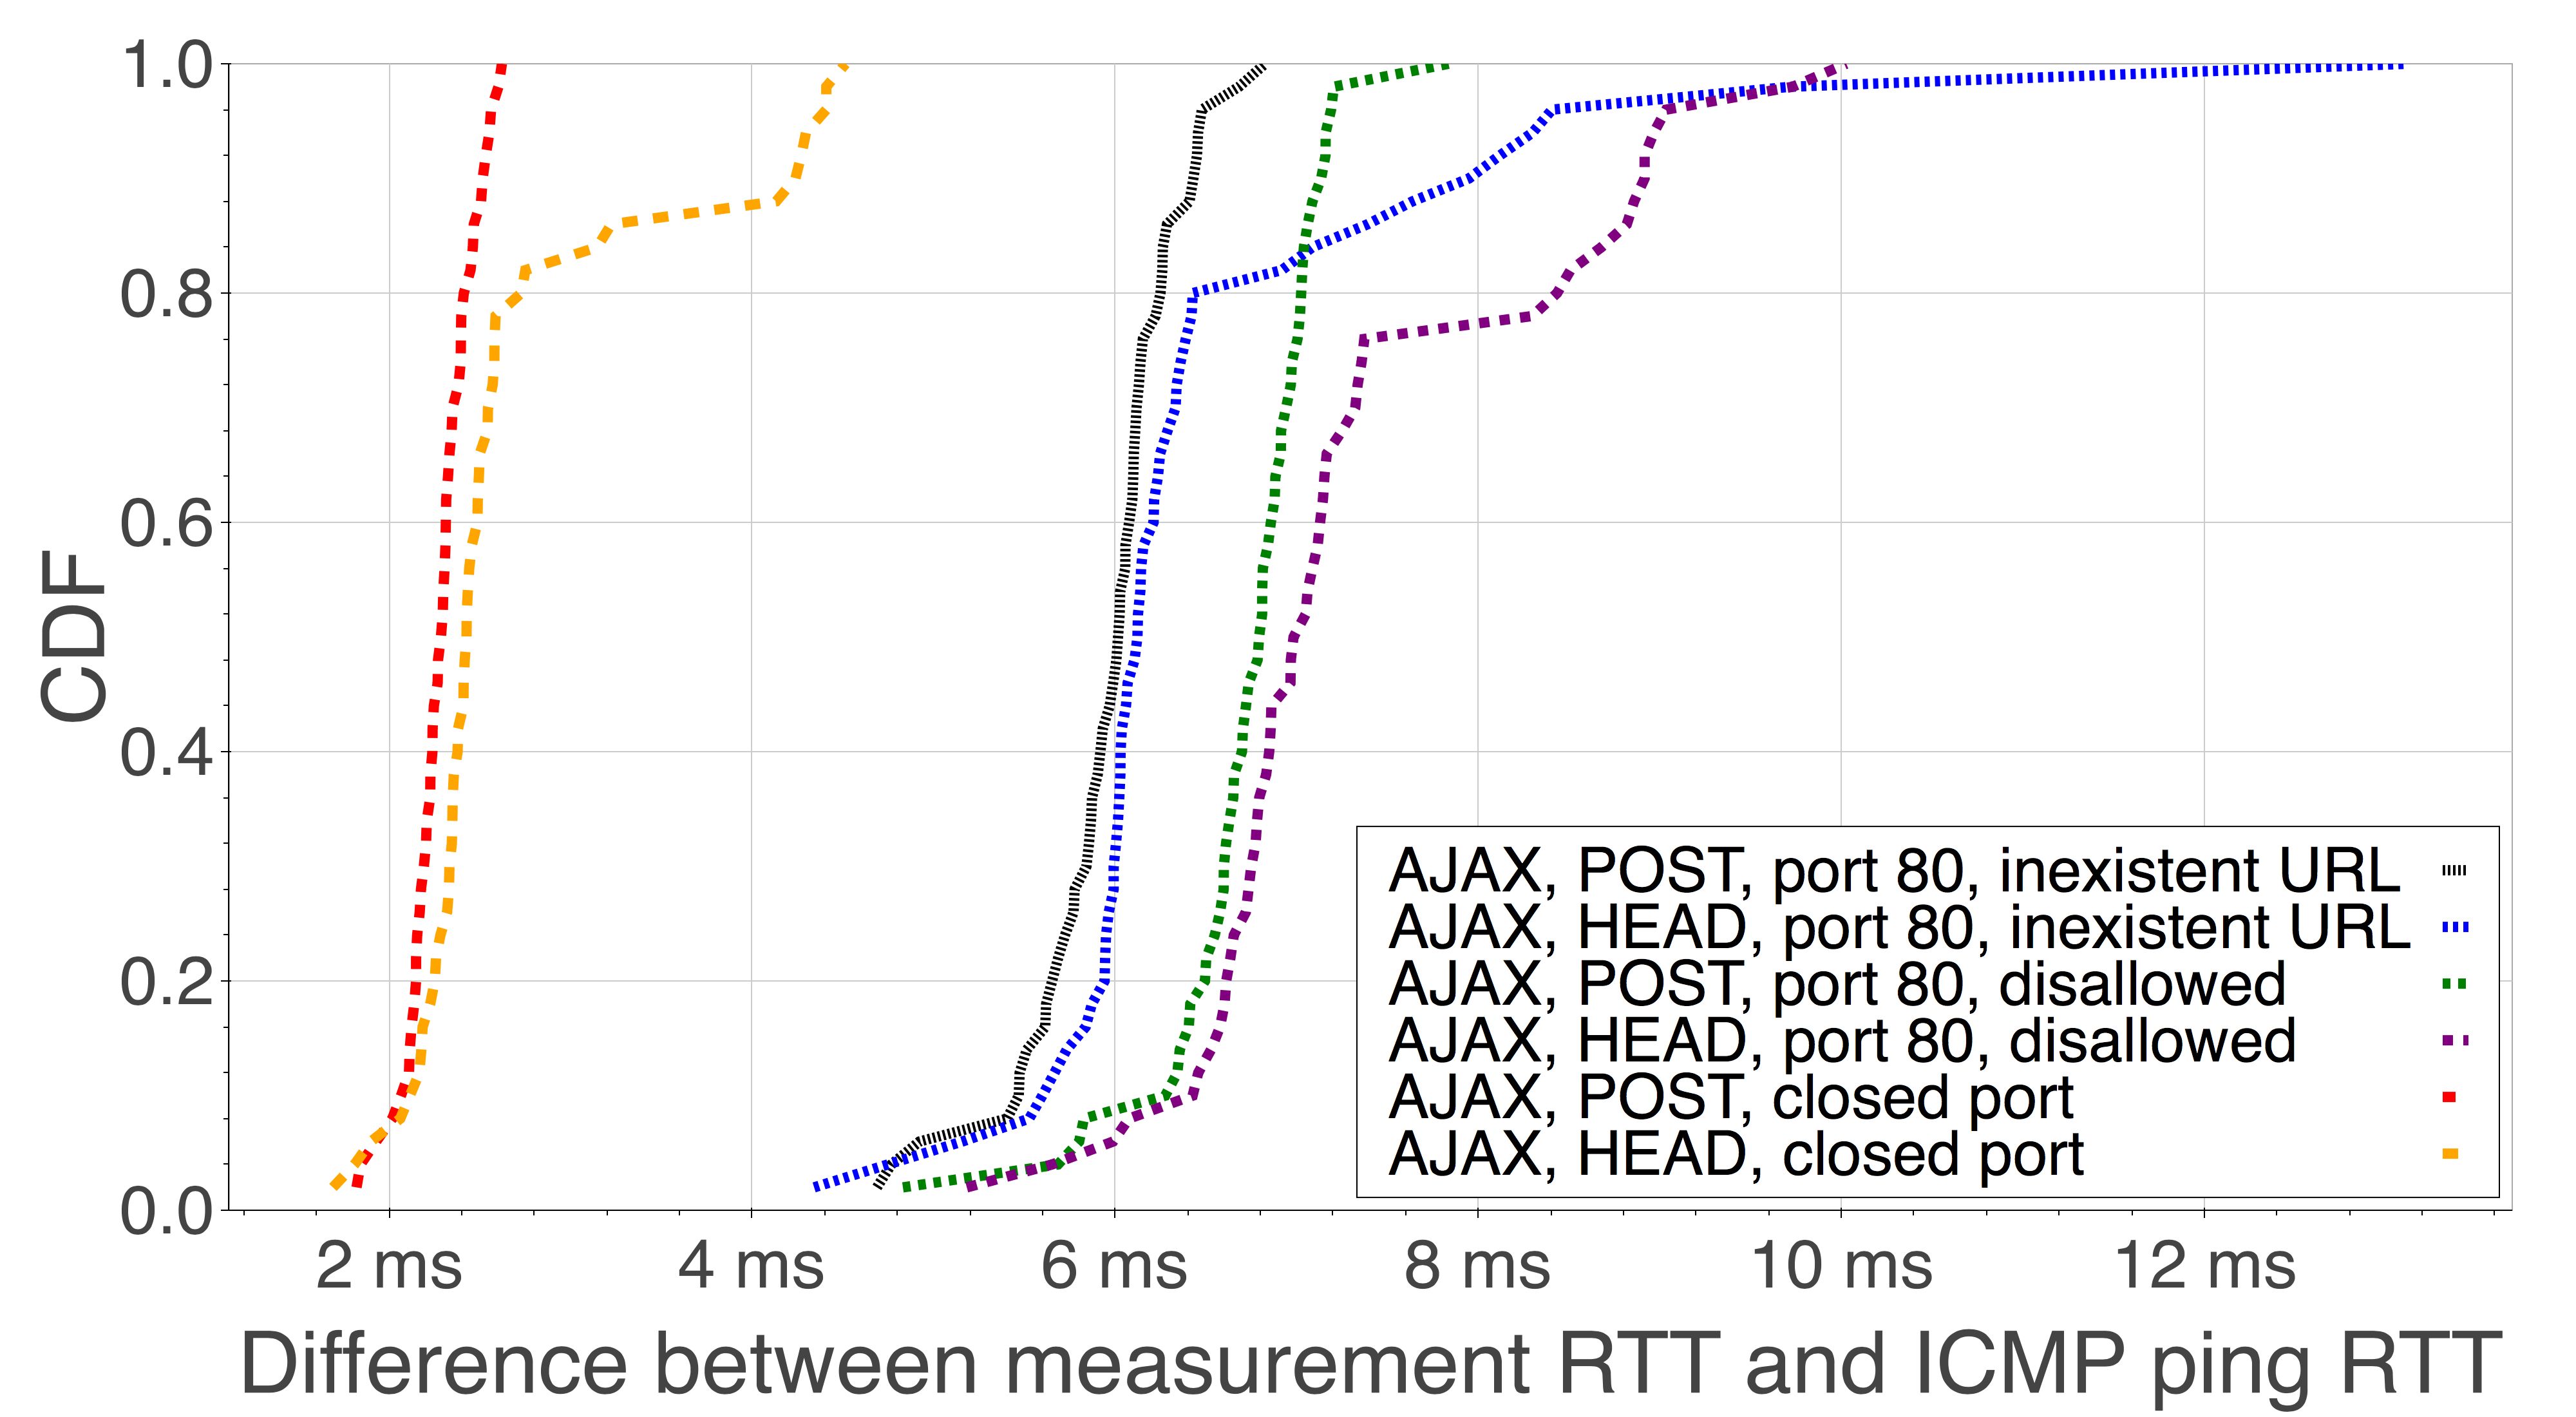
\includegraphics[width=\columnwidth]{figures/inet-non-coop-new}
\caption{Delay overheads to an uncooperative Internet target using AJAX (OS X/Chrome).}
\label{fig:inet_non_coop_new}
\end{figure}

In Figure~\ref{fig:inet_non_coop_new} we compare the different non-cooperative AJAX methods (inexisting URL, unallowed cross-origin request and a request to a closed port). We exclude HTTP GET as similarly to the cooperative case it performs generally worse than HEAD and POST. An AJAX request to a closed port shows the lowest overhead of around 2ms and is comparable, or even better in performance than the best cooperating methods (WebSocket and WebRTC). The invalid cross-origin request and access to non-existing resource have similar overhead, the former being slightly worse with around 7ms overhead in general. As in the cooperating server case, the request type has an impact on the overheads: POST has a slightly lower overhead than HEAD and similarly, POST has less variation in its overhead. Note also that the overhead from error response is smaller than the overhead when fetching an existing resource (order of 1ms). These results are similar for Firefox and across the operating systems.

\begin{figure}[h]
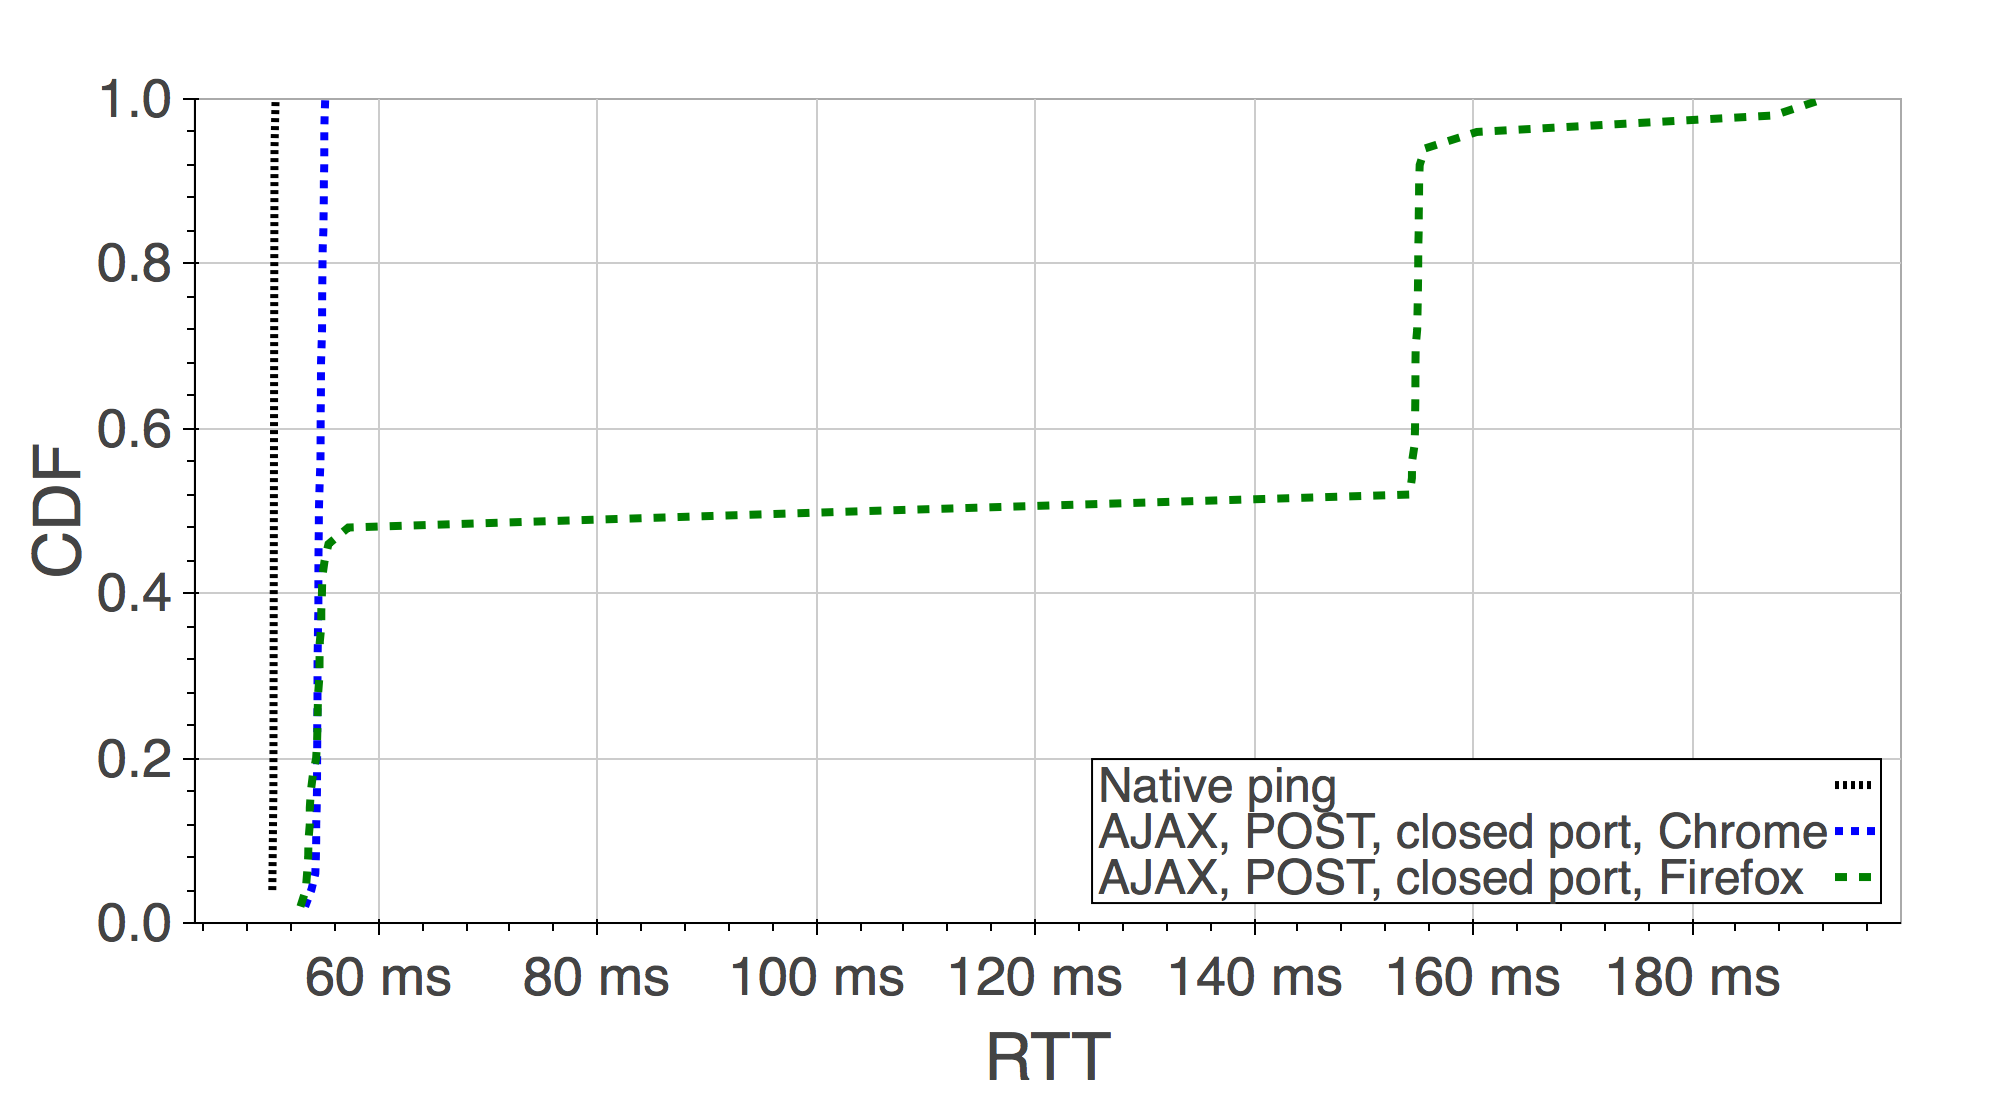
\includegraphics[width=\columnwidth]{figures/inet-comp-chrome-ff}
\caption{Delay overheads to an Internet server on a closed port (Ubuntu/Firefox, Chrome).}
\label{fig:inet_comp_chrome_ff}
\end{figure}

The AJAX request to a closed port seems attractive method for delay measurements. However, in practice it may be unusable due to the firewall problems discussed before. Even if the firewalls are not an issue, we observe another problem with the method. Namely, when requesting a page from a closed port on Firefox, the request does not always immediately return an error to our measurement code (\autoref{fig:inet_comp_chrome_ff}). The packet traces reveal that when Firefox gets an error after trying to contact a closed port, it retries up to three times and raises the error all the attempts failed. Furthermore, the method of sending AJAX requests to closed ports only works from an OS X or Linux host. Windows never immediately reports the connection refused error to an application upon receiving a RST packet but instead retries several times before quitting the connection attempt~\cite{r._jesup_info:_2011}, which makes this method unusable on Windows. 

%\subsubsection{Influence of Load}
%
%\begin{figure}[thb]
%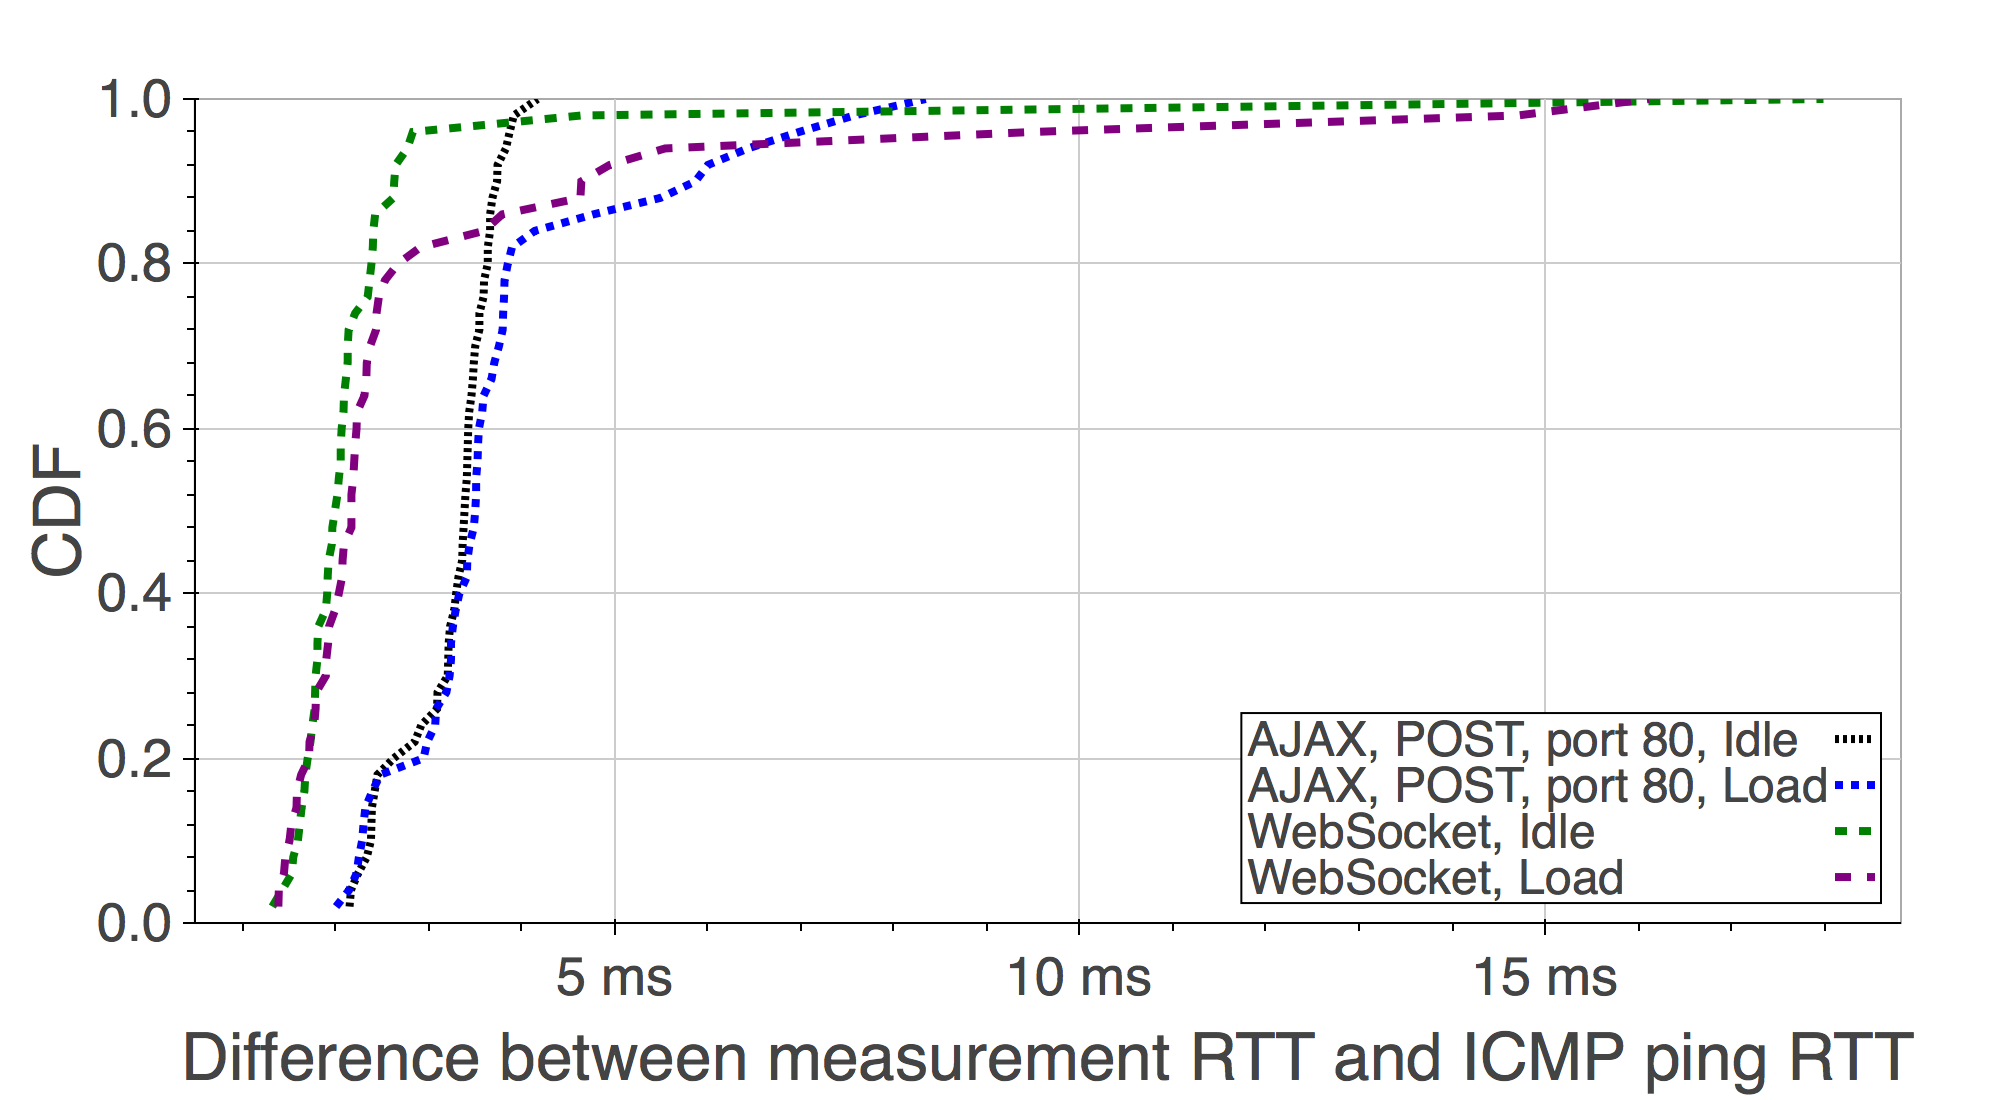
\includegraphics[width=\columnwidth]{figures/inet-comp-load-ff}
%\caption{Delay overhead to an Internet server when being idle or under load (Ubuntu/Firefox).}
%\label{fig:inet_comp_load}
%\end{figure}
%
%Figure~\ref{fig:inet_comp_load} compares the delay overheads of AJAX POST and WebSocket when the measurement client browser is under load or not. In general, the effect of load is higher variability in the overheads, the median cases remain the same. In general, Firefox is more impacted by load than Chrome where load has almost no effect, The results are consistent across all the methods and the three operating systems. We believe this might be caused by the multi-process architecture of Google Chrome~\cite{_multi-process_2008} where each web page runs in an independent process while in Firefox, currently, there is one process for all web pages and for the browser UI~\cite{_multiprocess_2016}.

\subsection{Local Network Delays}
\label{subsec:local}

In this section we focus on the local network delay measurements. The big challenge in measuring the delays in the local network is the overhead that in many cases is in the same order as the actual network delays.

\begin{figure}[thb]
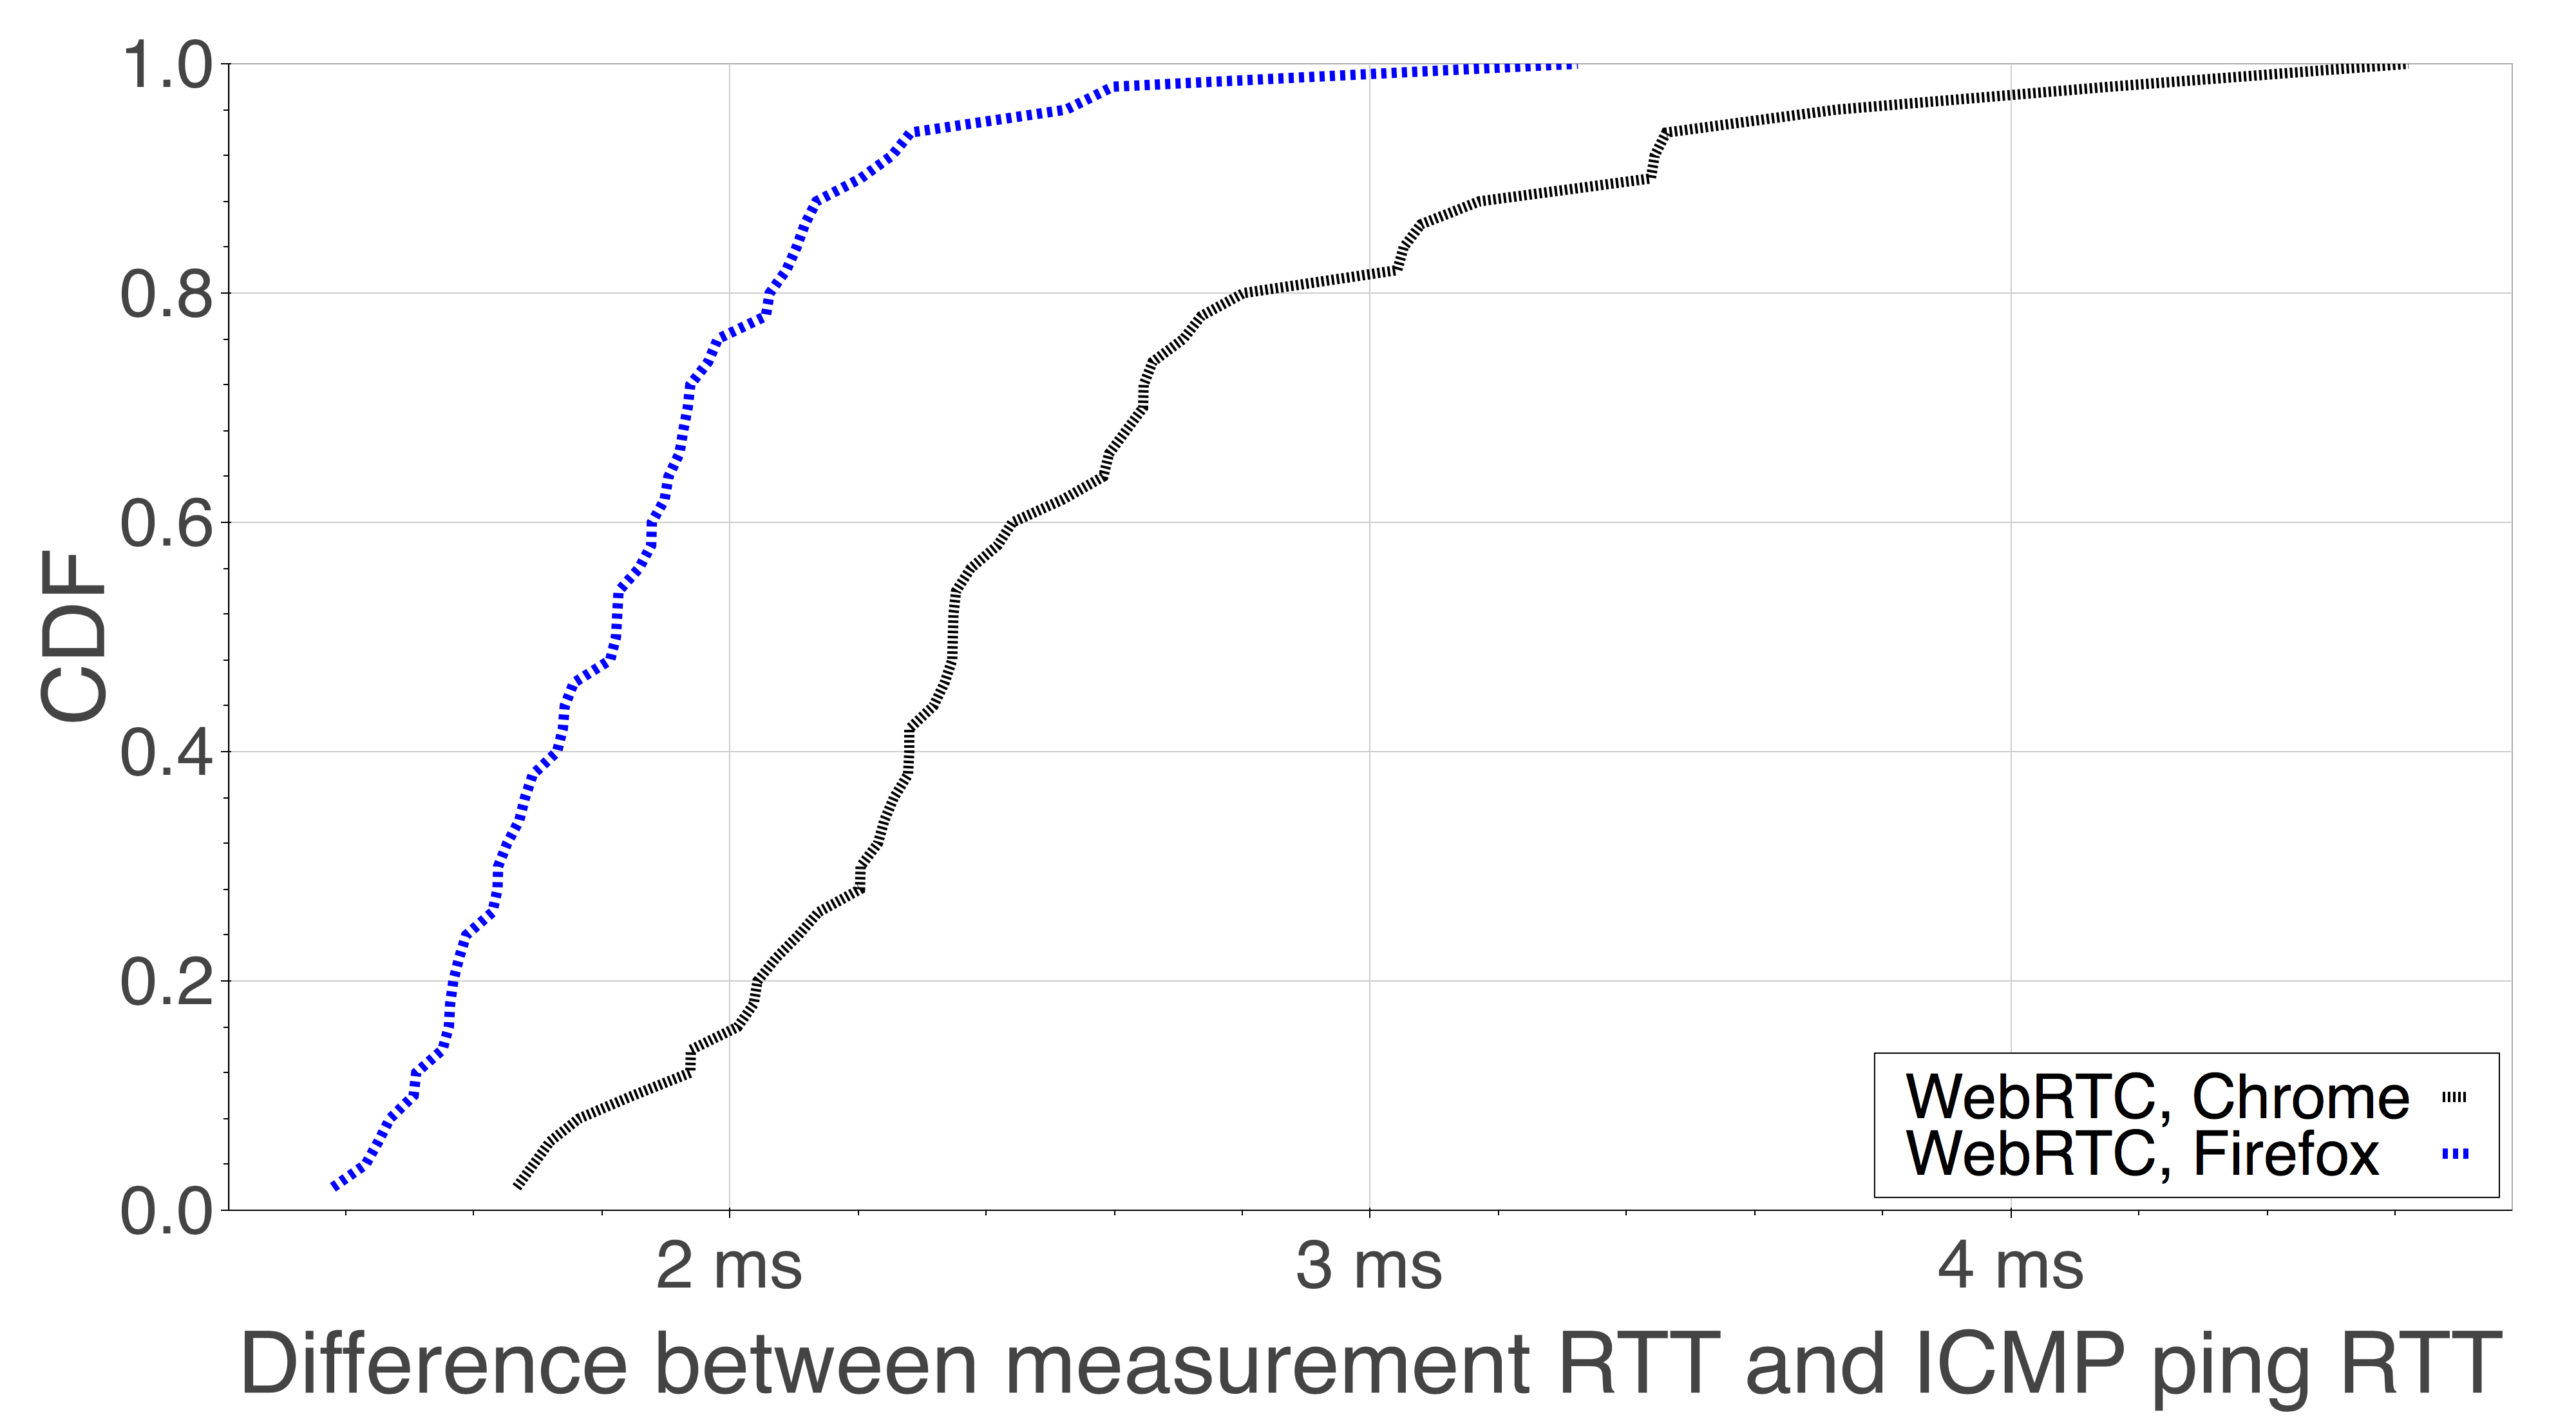
\includegraphics[width=\columnwidth]{figures/other-machine-comp-chrome-ff}
\caption{Delay overheads of WebRTC in local network (OS X/Chrome, Firefox).}
\label{fig:peer_comp_chrome_ff}
\end{figure}

We measure the delays to a peer device in the same local network using WebRTC and the results for OS X are shown in Figure~\ref{fig:peer_comp_chrome_ff}. The delay overhead is similar to the Internet server case discussed earlier, below 3ms for 80\% of the time for Chrome, and below 2ms for 80\% for Firefox. 

\begin{figure}[thb]
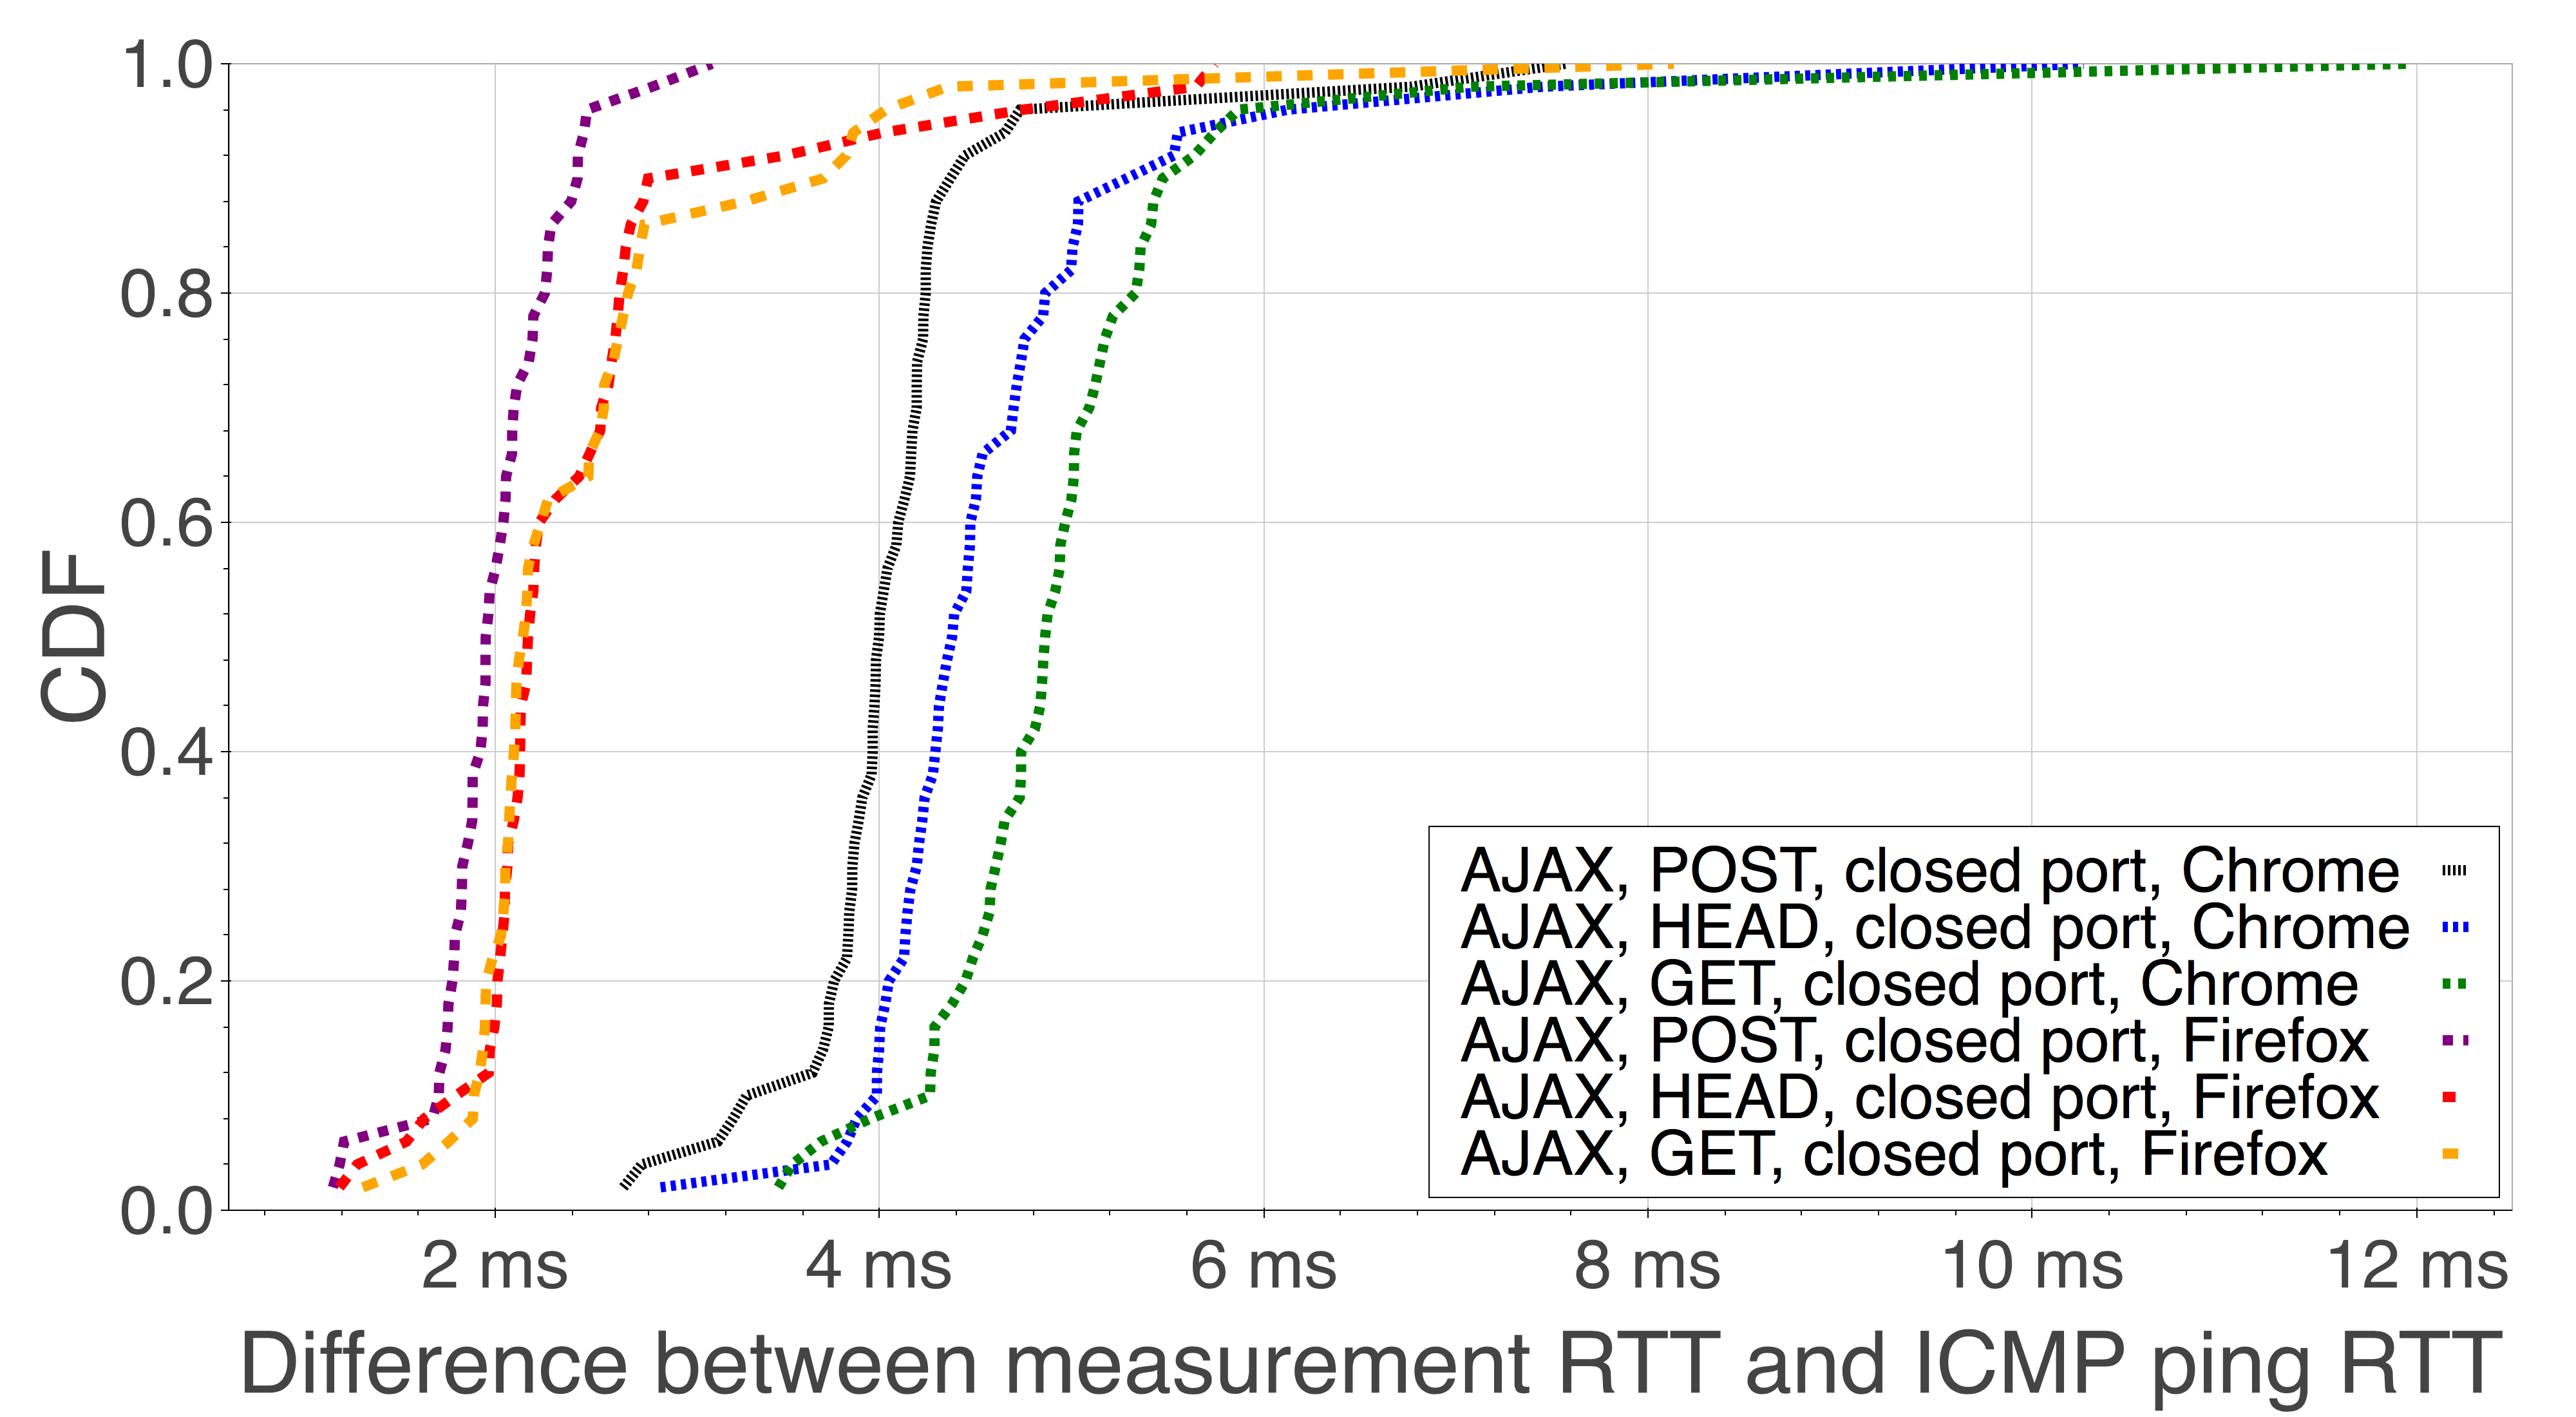
\includegraphics[width=\columnwidth]{figures/router-comp-chrome-ff}
\caption{Delay overheads to a home router (OS X/Chrome, Firefox).}
\label{fig:router_comp_chrome_ff}
\end{figure}

For the home router, we test various AJAX based methods. Figure~\ref{fig:router_comp_chrome_ff} compares the methods with the lowest overhead for Chrome and Firefox which is the various AJAX requests to a closed port (\emph{i.e.} we are basically measuring the TCP handshake delay). There is some variation between the different methods due to browser processing. This difference is particular large for Chrome. In general, the overhead is around 2ms for Firefox, and around 4ms for Chrome. 

Considering that the baseline delay of our local network setup is less than 1ms, the overheads for both peer device and router delay measurements are still high. However, our setup is basically testing the worst case as we connect everything via ethernet. Typical home networks are using mostly wireless connections, and especially in case of trouble, the wireless delays can be in the order of several tens of milliseconds.

\subsection{Conclusion}

%\todo[inline]{Delete this section completely?}

In this part, we explored the potential of using the web browser as a vantage point to measure RTTs from edge networks. 
%We perform controlled experiments from popular browsers and operating systems to study the overhead that browsers introduce when measuring RTTs in different scenarios. We compare several methods to measure RTTs---AJAX (HEAD, GET, POST), WebSocket, and WebRTC DataChannel. 
We first consider the case when the target is a cooperating server connected to the Internet. Our results confirm previous findings that in most cases WebSocket have the lowest overhead. WebSocket, however, sometimes introduce significant overhead (of 20~ms) making it an unreliable method to measure RTTs. Our experiments with WebRTC presented overheads that are only slightly higher than that of WebSocket but very consistent; making it the best choice for measuring Internet delays to cooperating targets. Then
we considered the case when measuring Internet delays to non-cooperating targets. We saw that opening an AJAX connection to a closed port introduces the lowest overhead, but it is not reliable on Firefox and on Windows. An alternative is to use AJAX to an inexistent URL. Finally, we considered cases where targets are in the local network. Both WebRTC between devices and AJAX to a closed port work well, but they introduce overheads around 2--4~ms. This is particularly challenging as the delays within local networks are in the same order as the measurement overhead browsers introduce. 

%\begin{table*}[t]
%\label{comparison}
%\centering
%\begin{tabular}{ll|ll|ll|ll}
%\noalign{\hrule height 1pt}
%\multirow{2}{*}{OS} & \multirow{2}{*}{Browser} & \multicolumn{2}{l|}{Router} & \multicolumn{2}{l|}{Other machine} & \multicolumn{2}{l}{Server} \\
%%\cline{3-8}
%&& Value & Method & Value & Method & Value & Method\\
%\noalign{\hrule}
%\multirow{2}{*}{OS X} & Chrome & 1.9 [1.8, 2.2] &Ajax Post, closed & 2.3 [1.7, 3.6] &WebRTC & 2.3 [2.0, 2.6]& WebSocket \\
%& Firefox & 3.1 [2.9, 3.4] &Ajax Get, closed & 1.8 [1.5, 2.4]& WebRTC & 2.4 [2.0, 3.5]& WebSocket\\
%\noalign{\hrule}
%\multirow{2}{*}{Ubuntu} & Chrome & 4.0 [3.3, 4.7] &Ajax Post, closed & 2.7 [2.2, 3.1]& WebRTC & 2.8 [2.5, 4.0]& WebSocket\\
%& Firefox & 2.0 [1.4, 2.5]& Ajax Post, closed & 1.8 [1.5, 2.1]& WebRTC & 2.4 [2.1, 7.1]& WebSocket \\
%\noalign{\hrule}
%\multirow{2}{*}{Win.} & Chrome & 3.7 [2.3, 4.3]& Ajax Post, inval.~path & 2.1 [1.4, 2.5]& WebRTC & 2.1 [1.6, 4.1]& WebSocket\\
%& Firefox & 3.3 [1.6, 3.7]& Ajax Post, inval.~path & 1.7 [1.0, 2.1]& WebRTC & 2.0 [1.5, 2.8]& WebSocket\\
%\noalign{\hrule height 1pt}
%\end{tabular}
%\caption {Measurement method with least overhead in milliseconds selected for each OS and browser by median in case of no additional load in the browser. 5th and 95th percentiles in brackets}
%\end{table*}

\section{Web based home network troubleshooting}

\label{sec:troubleshooting}

%\subsection{Introduction}

After having evaluated which web technologies are suitable for delay measurements in which contexts, the next step is to find a way to utilize these methods to measure users' home networks effectively and provide them with easily understandable feedback. 

\subsection{Objectives of a web based measurement tool}
\label{subsec:objectives}

First, it is necessary to define the specific goals of the web based measurement utility. The tool should perform a set of measurements to find out if there are bottlenecks in a user's home network such as
%\begin{enumerate}
%\item perform a set of measurements to find out if there are bottlenecks in a user's home network such as
\begin{enumerate}
\item a slow connection of a device to the home router (possible because of long distance too the router, interference etc.)
\item limited hardware performance impairs the measurement process and/or reduces available Internet speed
%\item (future work) insufficient hardware performance in the home router limits Internet speed
%\item (future work) an overloaded access link between the home router and the Internet Service Provider (ISP)
%\end{enumerate}
%\item (future work) inform the user about these problems (if there are any) and their severity in an easily understandable manner
%\item (future work) give the user instructions on how to resolve problems
%\item (future work) allow the user to compare his Internet connectivity performance to other users 
\end{enumerate}

As part of this thesis a prototype of a web page was developed which performs measurements and gives the user feedback about the performance of the user's end devices and the speed of the connection of each device to the home router. 
% The speed of the access link between the router and the ISP as well as the hardware performance of the router is currently not implemented. Furthermore, the utility does not inform the user about the reason of performance impairments and thus can also not give instructions on how to resolve potential problems.

\subsection{Workings of the prototype}
\label{subsec:workingsprototype}

When users want to measure their Internet connectivity they
\begin{enumerate}
\item visit the measurement web page in their browser, which features a button labeled ``start measurement''. The page shows a graph which depicts all other end devices in the same LAN on which the web page is opened, as well as the home router (labelled ``gateway'' as well as its IP address) and the connection to the Internet Service Provide (ISP, labelled ``Internet'') (see \autoref{fig:visualizationbw}).
\begin{figure}[tbh]
\begin{center}
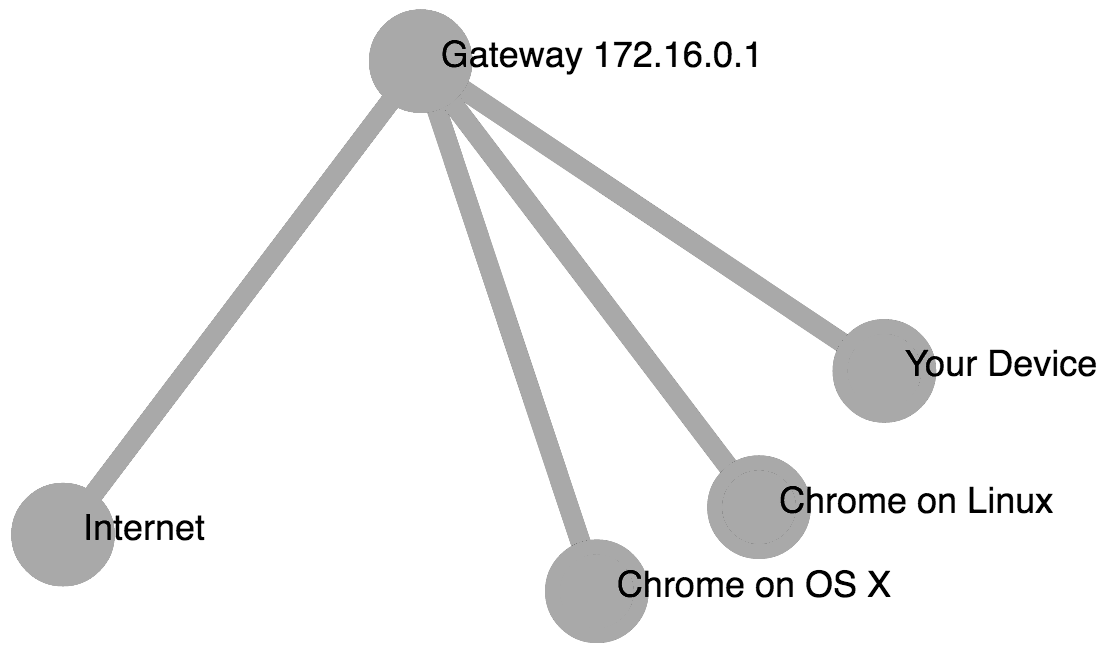
\includegraphics[width=\columnwidth]{figures/visualizationbw}
\end{center}
\caption{The visualization of the home network.}\label{fig:visualizationbw}
\end{figure}
\item press the button which launches the measurement
\item see the results after several seconds when the measurements are finished and evaluated (see \autoref{fig:visualization}). The prototype has two different kinds of visualizations, which use a continuous color from green over yellow and orange to red to indicate performance, where red means very bad performance and green means very good performance. 
\begin{figure}[tbh]
\begin{center}
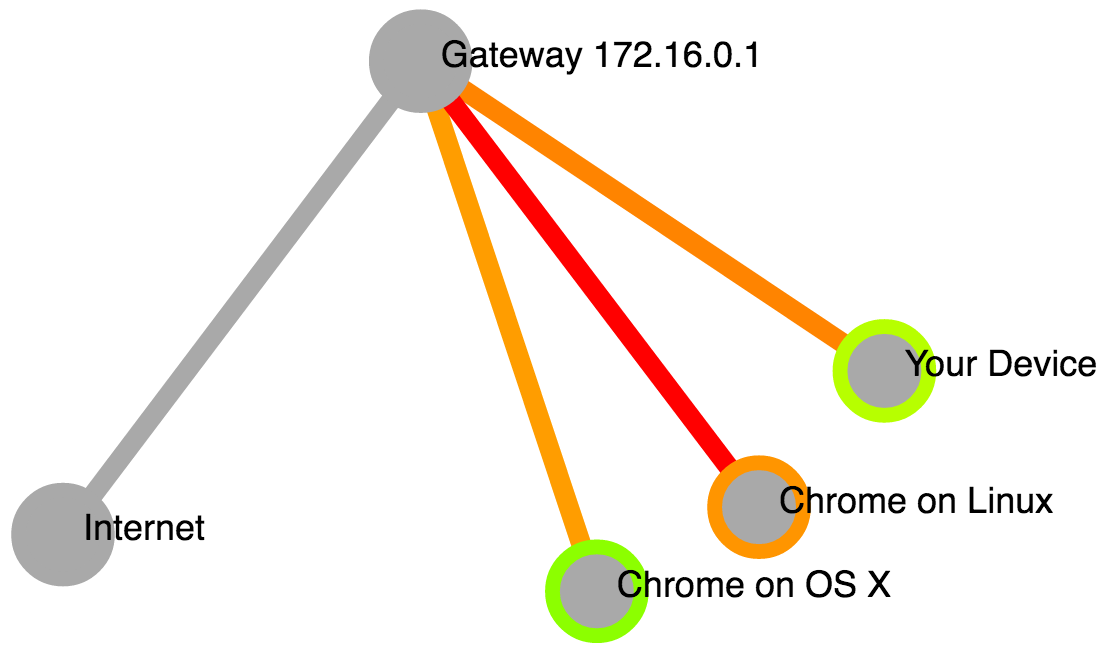
\includegraphics[width=\columnwidth]{figures/visualization}
\end{center}
\caption{The visualization of the performance in the home network.}\label{fig:visualization}
\end{figure}
\begin{enumerate}
\item The colored circle around each end device indicates the devices's performance and whether the device itself limits the network performance (e.g. because the device is overloaded with other tasks)
\item The colored line which connects each end device with the home router indicates the performance of the connection to the home router
\end{enumerate}
In the example in \autoref{fig:visualization} there are three end devices connected to the measurement web page in the LAN. The device named ``Your Device'' indicates the device from which the user starts the measurement. Due to security reasons, JavaScript cannot retrieve the name of the computer on which a web page runs and so instead the name of the web browser and the name of the operating system are chosen as approximate identifiers for the other end devices in the network (e.g. ``Chrome on OS X'' means that on this end device the measurement web page is opened using Google Chrome running on OS X).
\end{enumerate}

\subsection{Technical implementation}

A novelty of the prototype is its usage of WebRTC which allows a web page's JavaScript running on one machine to connect to any other web page running on another machine directly, if both parties are willing to establish the connection. To use WebRTC to allow a newly opened instance of the web page to connect to other existing instances of the measurement web page in the home network, first, the server, from which the measurement page was loaded, has to inform each instance of the web page first about the existence and address of the other instances in the home network. 

\subsubsection{Determining clients which are in the same home network}

To notify the new instance of the webpage in a home network about the other instances, the server first has to determine which instances of the measurement web page are actually colocated in the same home network. For determining whether two clients are in the same home network, there are two cases depending on whether the clients have IPv4 or IPv6 addresses. 

\paragraph{IPv4}When the server sees that the measurement webpage is opened several times from the same IPv4 address it can mean that (i) the web page is opened several times on the same machine or (ii) that it is opened on different machines behind a Network Address Translator (NAT) or (iii) it is a combination of both, e.g.~the web page is opened one time on machine \textit{A} and two times on machine \textit{B}. Irrespective of the case which applies, the web page is always opened in the same network when it is accessed several times from one IPv4 address. Thus, when several instances of the measurement web page share the same IP address it means that they are in the same home network.
%\todo[inline]{Add that it makes sense to filter when the web page is opened several times on the same machine because it makes weird interference.}

\paragraph{IPv6}Private end-users get /64 IPv6 subnets assigned by their residential ISP \cite{ripe_understanding_2015} and all end devices in a clients home network get assigned an IP address in the customer's /64 network. % using either SLAAC or DHCPv6. 
Thus, similar to the case of IPv4, if the measurement webpage is opened several times from within one /64 prefix and it belongs to a residential ISP, it can be assumed that the webpage is opened several times in the same LAN. 

\subsubsection{Establishing WebRTC connections}

When the server has determined all other instances of the web page opened in the same home network, it informs the new instance about the other instances and the new instance starts to set up the WebRTC connection. 

To set up a WebRTC connection between two clients, they must be able to communicate over a so-called ``signaling channel'', over which the clients can exchange information about their available IP addresses and other parameters of the prospective WebRTC connection. For the signaling channel we use WebSocket connections, which each instance of the web page maintains to the server. A client can send a message to another client in the same home network by sending it to the server which relays it to the client, which the message is addressed to. When the WebRTC connection is established, the clients set up a WebRTC DataChannel using the existing WebRTC connection \cite{k._drage_sdp-based_2016}. We choose to configure the DataChannel for unreliable and unordered transmission to be able to observer the number of lost packets and to make the DataChannel as transparent as possible (for more information about the DataChannel see \S\ref{subsubsec:webrtc}).

\subsubsection{Determining the home router's IP address}

Before starting a measurement, the clients must know the IP address of the home router because it is one of the measurement targets. 

\paragraph{IPv4}When clients in the network have IPv4 addresses, this usually means that the router uses DHCPv4 to allocate addresses and also has an IPv4 address itself. Usually one of the IP address spaces reserved for private usage is used (defined by the IEFT \cite{groot_address_1996}). By using WebRTC, all end devices in the network are able to retrieve their own private IP address in the network and the ones of all other peers. From the IP addresses of the devices in the network it is possible to deduce the subnet address which is used in the network. Commonly, home routers use the first available IP address in the subnet, so the router's IP address can be retrieved as being the first IP address in the subnet of the home network. In case the router does not use the first available address, it is possible to probe all IP addresses (in home networks commonly 254 available addresses) and check whether an HTTP server is running on port 80 of any of the available addresses, because home routers usually have configuration interfaces which are ran as web servers. Of course, also another device in the home network could run an HTTP server on port 80, however, it is not very likely for residential customers to have web servers running on their machines. The method to determine a router's IPv4 address is an heuristic and does not work for all possible configurations, however, it works for most common home network configurations.\\
As an example, if the router uses 192.168.0.0/24 (254 available IP addresses) as the network from which it assigns the IP addresses, the other devices would get assigned IP address like 192.168.0.25 and 192.168.0.124. When a device knows the IP addresses of the other devices it can assume that the router's IP address is 192.168.0.1, the first available IP address in the subnet. To check whether the assumption is true, one can try to contact the home router to determine whether a machine exists at the given IP address and one can try to access the router's HTTP interface at port 80. 

\paragraph{IPv6}If the client's network uses IPv6, NAT is usually not deployed \cite{zhang_iab_2010}. In this case the server can run a traceroute to the client which will determine all the IP addresses on the way to the client, including the router's IP address. The router's IP address is then the first one encountered with traceroute, which is in the same /64 network as the client. It might be the case that the router utilizes a firewall to limit filter incoming ICMP packets destined for clients in the home network. However, this case is irrelevant as only the trace of IP addresses up to the router is relevant and it is not necessary that we can actually reach the client itself with the traceroute. 
 Home routers have two IP addresses, one external one for their connection to the ISP and one internal one for the Wi-Fi interface over which the clients in the household are connected. This method retrieves only the external IP address because this is the only one which the server can see using traceroute. However, basically it doesn't matter which of the two IP addresses the client use as their measurement target. 

\subsubsection{The measurement process}

When the measurement web page is connected to all the other instances of the web page in the same network and the IP address of the router has been determined, measurements can be started. 

\begin{enumerate}
\item When the user pushes the ``Run measurement'' button, the measurement process is launched. 
\item The instance of the measurement web page prepares the request for measurement and randomly schedules all the instances in the home network to perform their measurements during different time intervals so that the measurements of the different instances do not interfere with each other. The measurement requests are then sent to each of the other instances in the same home network, including the instance, which initiated the measurement. 
\item Each instance of the measurement web page receives the instructions to perform measurements. They prepare for the measurements and wait for their scheduled time slot to perform measurements. 
\item When the scheduled time interval has arrived, the instance of the measurement web page simultaneously starts three different types of measurements over a duration of 2.5 seconds as a too long measurement process could frustrate users. The number of pings is chosen so that it does not overload the hardware and thus bias the measurement results.

\begin{itemize}
\item 151 RTT measurements using AJAX POST to a closed port of the home router
\item 151 RTT measurements using AJAX POST to the closest Measurement Lab server \cite{_measurement_????}
\item 501 RTT measurements using WebRTC to each of the peer instances of the measurement web page. 
\end{itemize}
Because the first measurement result of a sequence of measurements can be biased (see \S\ref{subsec:methods}), it is not considered for evaluation but dropped. 

When all peers are finished with the measurements they transmit the results to the instance of the web page which started the measurement process. Alongside the result the also send information about the operating system and the browser. 
\item The initializing peer receives the measurement results, aggregates them and transmits the results to the server for more detailed evaluation. 
%\todo[inline]{Maybe this stuff is irrelevant?}
\item Upon receiving the data and the information regarding the browser and the OS, the server saves it in a database, evaluates the results (see \S\ref{subsec:performancemethods}) and sends them back to the client which initialized the measurement. 
\item The client receives the evaluated results and graphically displays the results (see \S\ref{subsec:workingsprototype}).
\end{enumerate}

\subsection{Performance assessment methods}
\label{subsec:performancemethods}

When the server receives all the collected data of a measurement, it has to apply algorithms which estimate the performance of the links of each peer to the home router and which determine whether the devices themselves do not have sufficient performance to execute the measurements (see \S\ref{subsec:objectives}).

\subsubsection{Comparative approach}
\label{subsubsec:comparative}

The fundamental logic of the comparative approach is that if a user's measurements were worse than the ones of most other users, then quality is estimated to be bad. 

For this, the results of a user's measurements are compared to other users' results which were previously measured by Fathom and stored in a database. Fathom's dataset is used for comparison as it includes a vast and constantly growing number of measurement results. The data is filtered to only include measurements obtained over Wi-Fi connections because browser measurements performed over Wi-Fi cannot be compared to Fathom measurements done over Ethernet. However, it is not inherently necessary to depend on Fathom. In the future, when more data will have been collected using the measurement tool proposed in this thesis, also this data can be used for comparison. 

To avoid that measurements to the three different targets influence each other, the measurements are executed in random order. For example, 151 RTT measurements to the router are executed in 2.5s, and so the interval between the measurements is 2.5s/151 = 16.56ms. Each measurement is executed at a random time in this interval. The measurements to the device itself and the server are executed in the same timespan as the measurements to the router, but because of the randomness of their execution they cannot systematically influence each other. 

Because each measurement yields several datasets of results, a simplified notation is used in the following paragraphs: For example $m_r$ refers to the \textit{m}easurement results to the \textit{r}outer. $f_l$ refers to all the measurement results from the Fathom dataset which targeted the device itself (l for local). 

\paragraph{Performance of the link between device and router}

After finishing the measurements, a quality metric called $q_r$ is calculated from the measured data which is then compared to all other users' previous measurements in the Fathom database. Because the measurements performed by the measurement web page in the browser using JavaScript suffer from considerable overhead (see \S\ref{sec:delays}), but on the other hand Fathom uses native ping for its measurements, the measurement results obtained from browser based measurements cannot directly be compared with Fathom's results. 

To calculate $q_r$ three numbers are taken into consideration: The median RTT measured to the router ($\textsf{median}(m_r)$); the minimum RTT measured to the device itself ($\textsf{min}(m_s)$), which is assumed to be an estimate of the measurement overhead introduced by the browser; the ($\textsf{min}(f_l)$) minimum RTT to the device itself obtained from all data in the Fathom database, which were recorded on the same OS as the one where the measurement was performed. This is necessary as different OS might produce different RTTs to them measuring the delays to themselves. 

The router link quality metric $q_r$ is then calculated by first normalizing the $\textsf{median}(m_r)$ by subtracting $\textsf{min}(m_s)$ to remove the overhead introduced by the browser. As a second step, the minimum overhead from the Fathom dataset $\textsf{min}(f_l)$ is added to mak the normalized value comparable to the Fathom data. 

$$q_r = \textsf{median}(m_r) - \textsf{min}(m_l) + \textsf{min}(f_l)$$

%The idea is to take the measured RTT and "normalize" it by subtracting the overhead the browser adds (measured minimum RTT to self). The overhead of native ping, which Fathom uses, is added to make the value comparable to the Fathom dataset.

The router link quality $q_r$ is then percent-ranked in all the RTTs to Wi-Fi routers ever recorded by Fathom (where the Operating System is the same). The resulting number is in the range from 0\% (which means that $q_r$ reported a lower median RTT than all measurements in the Fathom database) to 100\% (all measurements in the database had lower RTTs than our current measurement) where 0\% is green and 100\% is red. 

\paragraph{Performance of device itself}

Besides the possibility that the connection to the home router suffers from inadequate performance, there is also the eventuality that the device itself is a performance bottleneck and Internet speed is decreased because CPU, memory or IO speed are insufficient. Analogously, a device quality metric $q_l$ is calculated as 

$$q_l = \textsf{median}(m_l) - \textsf{min}(m_l) + \textsf{min}(f_l)$$

and then ranked in all the Fathom data of measurements to the device itself. Also here, only values which were produced on the same OS are considered. 

Like for the quality to the router, it is not strictly necessary to use Fathom's data  as a reference, but also the data retrieved by the Web based measurement tool itself could be used. However, Fathom has a large amount of data collected ``in the wild'' already which makes it ideal for comparisons. 

\subsubsection{Statistical approaches}
\label{subsubsec:statistical}

While the comparative approach is very simple and delivers good results when it can make use of a large reference database, it also has some limitations. 

\begin{itemize}
\item While it is possible to use a sufficiently large reference database, such as Fathom, there is the problem that the population of households which contribute with their measurements to the Fathom database should have similar characteristics when compared to the population which performs the measurements with the browser based tool. It is likely that people who use Fathom are technically more versed than the general population and it might follow that they have Internet connections of different speed than the general population. 
\item If, on the other side, the data from users of the web measurement page itself is used, there might be a bias because people use troubleshooting tools often in case there is a problem (unlike Fathom which constantly measures in the background). Thus the database might fill with a too large proportion of ``bad'' measurement results which might distort results
\item As technology advances, Internet speeds increase and possibly RTTs decrease too. It might be a problem if, for example, a measurement performed in 5 years would be compared to data retrieved in 2016 as Internet speeds in 2016 are probably significantly lower than in 2021. 
\item RTTs are different for each browser and OS. Thus in a database the browser and OS which contributed each result must be noted. This makes data collection and comparability difficult. Also the fact that the OS and browser landscape changes over time shows the limitations of using a database. Furthermore, the question remains if it is possible to compare OS and browser different versions with each other or not. 
\end{itemize}

From these limitations it follows that it might be preferable to use an approach which is independent of an external database because it ensures that the web based measurement tool will work equally well on all OS and browsers and also will not produce distorted results due to possible issues with the reference data. Furthermore, as it does not use a reference database, the overheads added by the browser are not so critical anymore, since the data is only compared to data from the same browser itself, not to other results.

The concept behind the statistical approach is to perform repeated measurements to three targets: an Internet server, the home router and the device itself. In each measurement round RTT measurements to the three targets are performed at exactly the same time. After a sufficiently large number of successful measurements, linear regression is used to determine whether the RTT measured to the router and to the device itself influences the RTT to the Internet server. The \textit{coefficient of determination} (also known as $r^2$), which is a number ranging from 0 to 1, is then used to assess how much the connection to the router and potential performance issues in the device itself are impairing the Internet connection.

\paragraph{Performance of the link between device and router}

To indicate whether the wireless connection is an actual bottleneck, linear regression is performed after the measurements are finished and $r^2$ is inspected. In case $r^2$ is 1.0 it would mean that all variance of delay observed for the Internet server can be attributed to variances of delays in the home network. This would mean that the wireless delays would fully predict the delays to the server. Intuitively one might think that this happens in the case of a bad wireless connection as then delays in the wireless link highly influence the connection to an Internet server. Conversely, in case of an excellent Wi-Fi connection one would expect the delays to the router and in Internet server to be largely unrelated. 

For visualization, $r^2$ = 0 would be displayed as a green link to the router while $r^2$ = 1 would be red. 

\paragraph{Performance of device itself}

Just as for the performance of the link to the router, for the performance of the device itself, linear regression is performed between the RTT to the server and the RTT to the device itself. The resulting $r^2$ can then be used for coloring. 

\subsection{Evaluation}

In \S\ref{subsubsec:statistical} we proposed a new method to determine the quality of wireless links based on the hypothesis that delay measurements performed to the device itself, the home router and an Internet server at the same time correlate in case of insufficient device performance or bad wireless connection and that Wi-Fi delays can predict the server delays. 

\subsubsection{Experimental setup}

In order to verify these hypotheses, we conducted a controlled experiment. The two cases of excellent Wi-Fi condition (client placed next to the access point) and bad Wi-Fi connection (client was placed far away from the router with low signal) were tested once under load and once idle.

The home router was connected with a 100~MBit/s connection to the Internet. The server in the Internet used for the delay measurements was 5 hops away from the client. The client was a laptop running \textit{OS X}. The load was generated using four concurrent programs which read random data from \texttt{/dev/urandom} and compressed it using \textit{bz2}. 

For all scenarios 1000 measurement rounds to an Internet server, the home router and the device itself were performed, every 250ms, using native ICMP ping. Then linear regression was performed to determine whether the delay in the home network or the delay to the device itself influence the delay to the Internet server. 

\subsubsection{Results}

\begin{table*}[htb]
\
\noindent\makebox[\textwidth]{%
\begin{tabular}{lllll}
\toprule
\textbf{Scenario} & \textbf{self} & \textbf{router} & \textbf{router \& self} \\
\midrule
Good Wi-Fi, no load & 0.0012 & 0.0137 & 0.015 \\
Bad Wi-Fi, no load & 0.0063 & 0.8428 & 0.8438 \\
Good Wi-Fi, load & 0.0024  & 0.1617 & 0.1654 \\
Bad Wi-Fi, load & 0.025 & 0.815 & 0.8159 \\
\bottomrule
\end{tabular}
}
\caption {$r^2$ in case of good Wi-Fi and bad Wi-Fi, with and without load} 
\label{tab:statistical}
\end{table*}

In \autoref{tab:statistical} for each scenario $r^2$ was calculated \begin{enumerate}
\item considering how well the delay to the device itself predicts the delay to the server
\item considering how well the delay to the router predicts the delay to the server
\item considering how well the delay to the device itself and the router predicts the delay to the server 
\end{enumerate} 

\begin{figure}[tbh]
\begin{center}
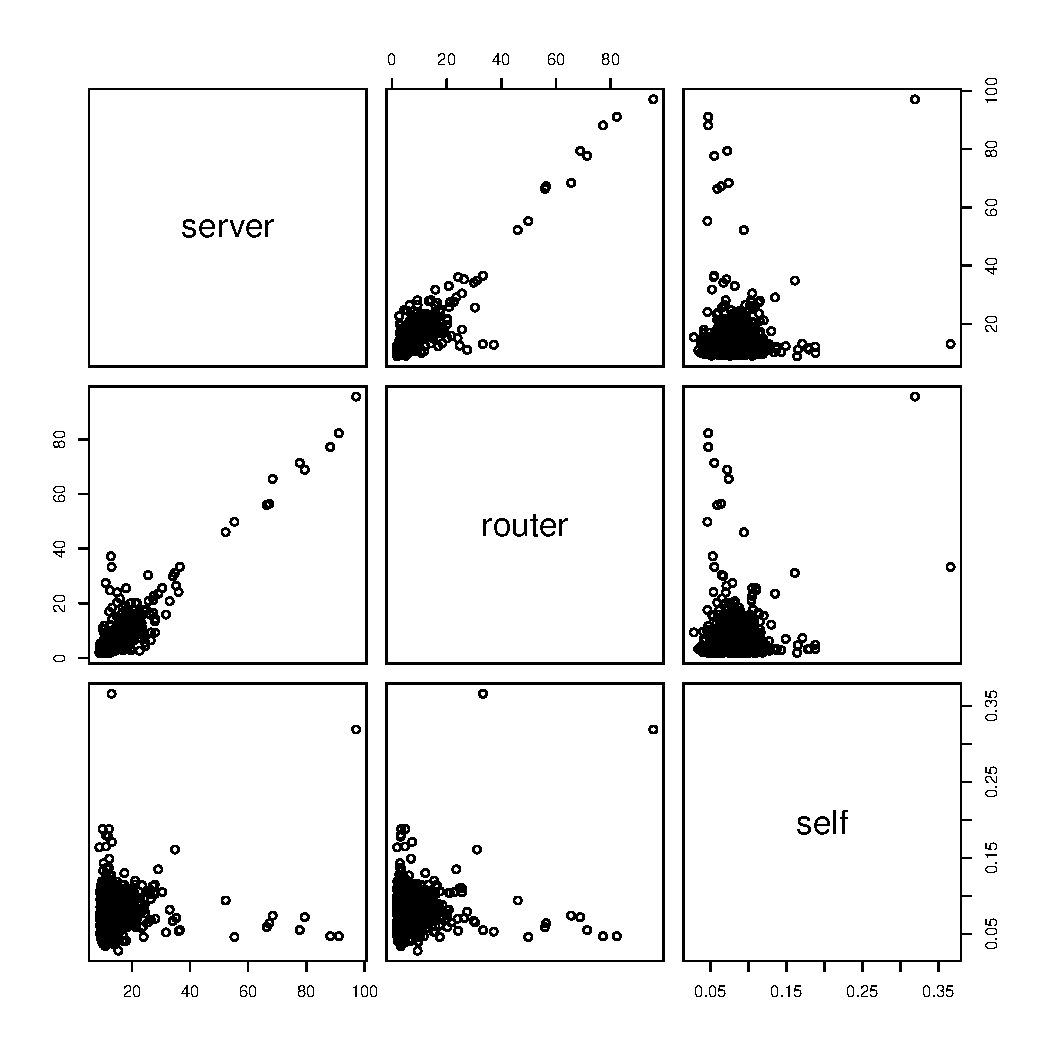
\includegraphics[width=\columnwidth]{figures/Rplots_bad_new}
\end{center}
\caption{Scatterplot showing RTT in milliseconds to server, router and the device itself in case of bad Wi-Fi and no load}\label{fig:badwifi}
\end{figure}

In case of good Wi-Fi we can see that neither \textit{self}, \textit{router} nor both combined can predict delays to the server. On the other side, in case of bad Wi-Fi we can see that while \textit{self} still cannot predict Internet delay, \textit{router} accounts for 84\% of observed variance in delay seen to the Internet server (see \autoref{fig:badwifi}). Thus we can conclude that the statistical approach is a suitable way of discovering throughput bottlenecks at least when they are caused by a slow wireless connection. 

We can see that load does not have a large influence on the relationship between the delay to the device itself and the delay to the server. However, it has a small but significant influence on the delay to the router. A possible reason for this could be the fact that more CPU time is required to send packets over a real physical interface when compared to the loopback interface which is used when sending packets to the device itself. 

\section{Conclusion}

The goal of this thesis was to find approaches which enable to perform home network troubleshooting based on web browsers, using recent web technologies. An important part of this is to detect whether problems with the wireless link could be the reason of insufficient Internet performance and to inform the user about these potential problems using an easy to understand visualization. 

To accomplish this goal, first, related work regarding web based measurements was reappraised and several new web technologies were tested for their feasibility to perform delay measurements from the browser. 

Second, based on the obtained results, suitable delay measurement techniques were chosen and a prototype of a web page was developed which can perform measurements in a home network. This prototype includes a simple visualization depicting the devices in the home network as a graph and visualizing the speed of the various components. 

Two approaches were developed to evaluate performance in the home network:
\begin{itemize}
\item The comparative approach which uses measurement results to compare them to a database of previously recorded values and judges quality based on the relative performance of these previous measurements. 
\item The statistical approach bases on the hypothesis that in case of bad wireless performance, the delay measured to the Wi-Fi router predicts the delay measured to an Internet server. To test this hypothesis, an evaluation was carried out which confirms our assumption and implies that the statistical approach is a promising method that can be used for home network troubleshooting. 
\end{itemize}

\section{Future work}

In this thesis we only used the statistical approach to determine whether components in the home network are a reason for low Internet speed seen by a particular client. Besides only carrying out linear regression for one client device, it would also be interesting to compare measurements executed by several devices at the same time and then use regression and other means of analysis to verify whether only one device is suffering from impaired wireless quality or all devices together. One potential problem with this idea is the fact that the statistical approach requires delay measurements to be executed at exactly the same time. Thus it would be necessary to have synchronized clocks in the range of one millisecond.

Furthermore it would be interesting to verify whether the statistical measurement approach can also be applied to cellular connections. This would allow to determine whether mobile users face slow internet connections due to the wireless connection to the base station or because the backbone network of the ISP is overloaded. 

%\phantomsection
%\addcontentsline{toc}{section}{Bibliography}

%\printbibliography
\bibliographystyle{abbrv}
\bibliography{thesis}

% That's all folks!
\end{document}
